\def\filedate{2010-08-09}\let\thedate\filedate % packages may change \filedate

\documentclass[twoside]{article}
\usepackage{ucs}\usepackage[utf8x]{inputenc}
\usepackage{natbib}
\usepackage{chem}
%\usepackage{afterpage}
\usepackage{url}
\usepackage{color}
%\usepackage{multicol}
\usepackage{rotating} % loads graphicx
%\usepackage{longtable}
\usepackage{graphicx}
%\usepackage{eclclass}
%\usepackage{verbatim}

% activate to show "draft" watermark:
\usepackage{draftcopy}

\oddsidemargin0mm
\evensidemargin-10mm
\topmargin-10mm
\textheight235mm
\textwidth175mm
\raggedbottom
\parindent0mm
\parskip1.0ex plus0.5ex minus0.5ex
\renewcommand{\arraystretch}{1}
\renewcommand{\topfraction}{0.95}
\renewcommand{\dbltopfraction}{0.95}
\renewcommand{\bottomfraction}{0.95}
\renewcommand{\floatpagefraction}{0.9}
\renewcommand{\dblfloatpagefraction}{0.9}
\renewcommand{\textfraction}{0.1}
\setcounter{topnumber}{3}
\setcounter{bottomnumber}{3}

\newcommand{\todo}[1]{{\uppercase{\bf ((#1))}}}
\newcommand{\egcite}[1]{\citep[e.g.][]{#1}}

\def\nosep{\setlength\parsep{0mm}\setlength\topsep{0mm}\setlength\itemsep{0mm}}

\def\mypageheader{Sander et al.: CAABA/MECCA User Manual}
\markboth{\mypageheader}{\mypageheader}
\pagestyle{myheadings}

% This file was created automatically by xmecca, DO NOT EDIT!
% xmecca was run on 2010-08-26 at 14:15:43 by caaba
\def\meccaversion{\code{2.7b}}
\def\kppversion{\code{2.2.1_rs5}}
\def\wanted{\code{Tr && G && !S && !Cl && !Br && !I && !Hg}}
\def\apn{0}
\def\gasspc{448}
\def\aqspc{0}
\def\allspc{448}
\def\Geqns{246}
\def\Aeqns{0}
\def\Heqns{0}
\def\Jeqns{72}
\def\HETeqns{0}
\def\EQeqns{0}
\def\IEXeqns{0}
\def\Deqns{0}
\def\alleqns{318}
 % \def\meccaversion{...}

% line break after \paragraph:
\makeatletter
\renewcommand\paragraph{\@startsection{paragraph}{4}{\z@}%
  {-2.0ex\@plus -1ex \@minus -.2ex}%
  {1.0ex \@plus .2ex}%
  {\normalfont\normalsize\bfseries}}
\makeatother

\begin{document}

\thispagestyle{empty}

\begin{center}
  
\includegraphics[height=0.3\textheight]{caaba_mecca_logo_print}\\[10mm]
  {\Huge\bf CAABA/MECCA-{\meccaversion} User Manual}\\[10mm]
  {\huge\em \underline{C}hemistry \underline{A}s \underline{A}
    \underline{B}oxmodel \underline{A}pplication /}\\[3mm]
  {\huge\em \underline{M}odule \underline{E}fficiently
    \underline{C}alculating the\\[5mm]
    \underline{C}hemistry of the
    \underline{A}tmosphere}\\[10mm]
  {\huge\bf Rolf Sander, Hartwig Harder, Patrick J\"ockel, Astrid
    Kerkweg \& Hella Riede}\\[15mm]
  \Large
  Air Chemistry Department\\
  Max-Planck Institute of Chemistry\\
  PO Box 3060, 55020 Mainz, Germany\\
  \url{sander@mpch-mainz.mpg.de}\\[10mm]
  {\huge\url{www.mpch-mainz.mpg.de/~sander/messy/mecca/}}
  \vfill
  Date: \thedate
\end{center}

\clearpage

\setlength{\columnsep}{8mm}
\twocolumn\sloppy

\tableofcontents

\begin{figure*}%[htb]
  \begin{center}
  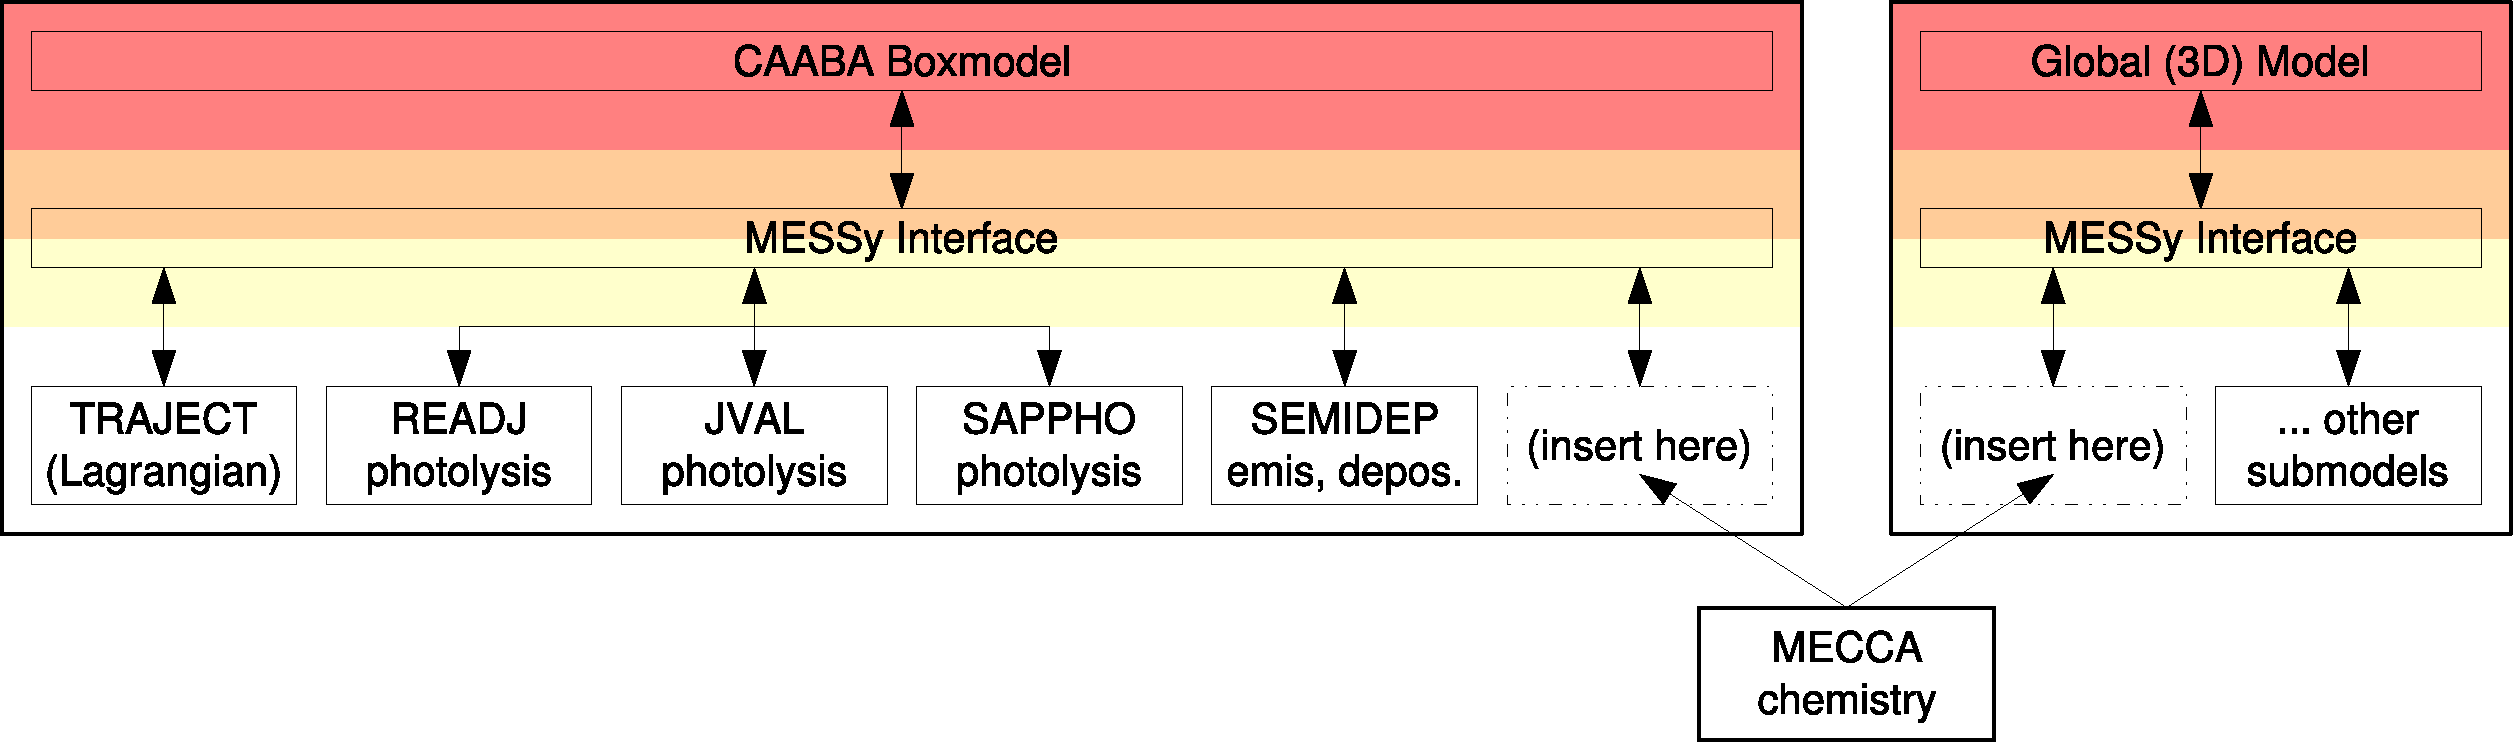
\includegraphics[width=0.9\textwidth]{modular-mecca}
  \end{center}
  \caption{Diagram showing MECCA as part of the CAABA box model or of a
    global model.}
  \label{fig:modular-mecca}
\end{figure*}

\section{Introduction}

MECCA (\underline{M}odule \underline{E}fficiently
\underline{C}alculating the \underline{C}hemistry of the
\underline{A}tmosphere) is an atmospheric chemistry module that contains
a comprehensive chemical mechanism with tropospheric and stratospheric
chemistry of both the gas and the aqueous phase \citep{1666,2405}. For
the numerical integration, MECCA uses the KPP software \citep{1665}.

To apply the MECCA chemistry to atmospheric conditions, MECCA must be
connected to a base model. As shown in Fig.~\ref{fig:modular-mecca}, the
base model can be a complex, 3-dimensional model \egcite{1851} but it
can also be a simple box model. The connection is established via the
MESSy interface (\url{http://www.messy-interface.org}) developed by
\citet{1664}.

This manual describes how to install and work with MECCA when it is
connected to the box model CAABA (\underline{C}hemistry \underline{A}s
\underline{A} \underline{B}oxmodel \underline{A}pplication). This
combination will be referred to as ``CAABA/MECCA''. The main features of
the CAABA box model are shown in Fig.~\ref{fig:caaba_sketch}. In
addition to MECCA chemistry, CAABA also contains several other
submodels, e.g.\ JVAL for calculating J-values, SAPPHO for simplified
and parameterized photolysis rates, and SEMIDEP for simplified emission
and deposition.

\section{Installation}
\label{sec:install}

This section can be skipped if CAABA/MECCA is already installed on your
computer.

\subsection{System Requirements}

\subsubsection{Linux/Unix}

CAABA/MECCA has been tested successfully on several UNIX-like operating
systems. The easiest installation is probably on a Linux PC since
several auxiliary programs are already included in a typical Linux
distribution. 

\subsubsection{MAC OS X}

CAABA/MECCA does not work with the version of the \verb|sed| program
that is shipped with MAC OS X. Instead, it is necessary to install the
GNU version of \verb|sed|, called \verb|gsed|. This can be done using
the MacPorts (\url{http://www.macports.org/}). To ensure that
\verb|gsed| is always executed when \verb|sed| is called, a symbolic
link from \verb|sed| to \verb|gsed| can be created, e.g.:
\begin{verbatim}
sudo ln -s /opt/local/bin/gsed
  /opt/local/bin/sed
\end{verbatim}

\subsubsection{Windows}

A native installation under Windows is neither recommended nor
supported. However, it is possible to run the model in a virtual Linux
machine on a Windows PC.

\todo{add more text based on info from hartwig here}

\subsection{Prerequisites}

\begin{description}
\item[A Fortran90 compiler (mandatory):] Several compilers have been
  tested successfully: g95 (for Linux), Lahey (for Linux), Intel (for
  Linux), Compaq (Alpha UNIX). Other compilers can be used as well if
  they accept standard Fortran90 code. It should be noted that the g95
  compiler for Linux is free and can be downloaded from
  \url{http://www.g95.org/}.
\item[The Kinetic PreProcessor KPP (mandatory):] This flexible numerical
  integration package by \citet{1665} transforms the chemistry mechanism
  into a set of ordinary differential equations (ODEs) in Fortran90
  syntax. MECCA needs the KPP version that is provided in the
  \verb|mecca/kpp/| directory. Follow the instructions in
  \verb|mecca/kpp/readme| to install KPP.
\item[Perl, tcsh, awk, sed, and make (mandatory):] These UNIX tools are
  standard on Linux systems. Check that recent versions of them are
  installed. Especially awk may lead to strange error messages.
  To test awk, type:\\
  \verb|awk 'BEGIN {print match("X","[^a-z]")}'|\\
  The result should be ``1''. However, you may get ``0'' as the result
  on your system. Supposedly, this is not a bug in awk but a feature.
  You can solve the problem by setting the environment variable
  \verb|LC_ALL| to ``\verb|C|'':\\
  \verb|export LC_ALL=C| $\qquad$ (if you use bash)\\
  \verb|setenv LC_ALL C| $\qquad$ (if you use tcsh)\\
  When you try the awk test again, it should work fine.
\item[La\TeX\ (optional):] If you have La\TeX\ installed on your
  computer, you can print a table (including rate coefficients and
  references) of the currently selected mechanism (see
  Sect.~\ref{sec:latextable} for details).
\item[netCDF library (optional):] The netCDF library is needed to create
  model output in netCDF format. It can be obtained from
  \url{http://www.unidata.ucar.edu/software/netcdf/}. Note that several
  files in the netCDF library are compiler-specific. Thus, it is
  necessary to create a netCDF library for each compiler and maybe also
  for each compiler version.

  Software for manipulating or displaying netCDF data is listed at:
  \url{http://www.unidata.ucar.edu/software/netcdf/software.html}. If
  you don't have the netCDF library, you can still run the model but
  produce only ASCII output.
\item[netCDF tools (optional):] Several tools are used to analyse the
  netCDF output when the model is run in the multirun
  (Sect.~\ref{sec:multirun}) or Monte-Carlo (Sect.~\ref{sec:montecarlo})
  mode. Specifically, the NCO programs \verb|ncpdq|, \verb|ncrcat|, and
  \verb|ncks| from \url{http://nco.sourceforge.net} and the program
  \verb|ncclamp| from \url{http://ncclamp.sourceforge.net} are needed.
\item[ferret (optional):] The ferret plotting program is needed to plot
  the contents of the netCDF output using the ferret scripts in the
  \verb|jnl/| directory (see Sect.~\ref{sec:ferret} for details). To
  ensure that ferret finds all necessary files, you have to add
  ``\verb|./tools|'' to the \verb|FER_GO| environment variable. The
  \verb|ferret_paths*template| files show how to do this. For example,
  when using the tcsh, type:\\
  \verb|setenv FER_GO "$FER_GO ./tools"|
\end{description}

\begin{figure*}%[htb]
  \begin{center}
  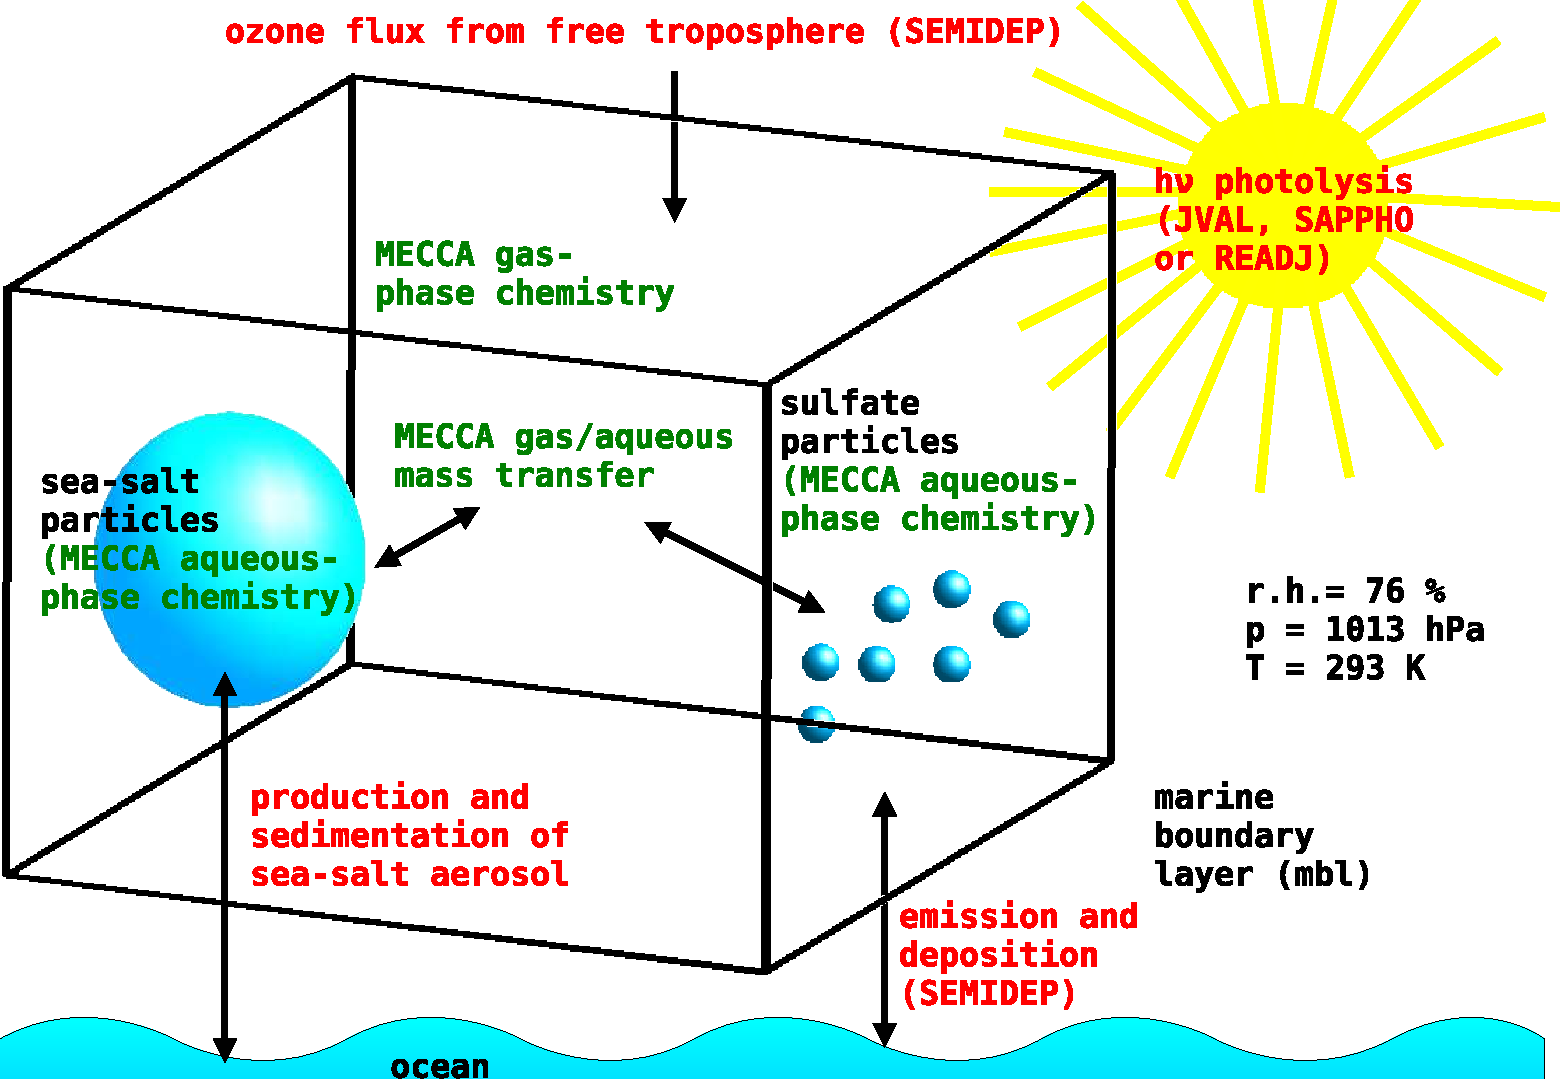
\includegraphics[width=0.9\textwidth]{caaba_sketch}
  \end{center}
  \caption{The CAABA box model}
  \label{fig:caaba_sketch}
\end{figure*}

\begin{figure*}
  \begin{center}
    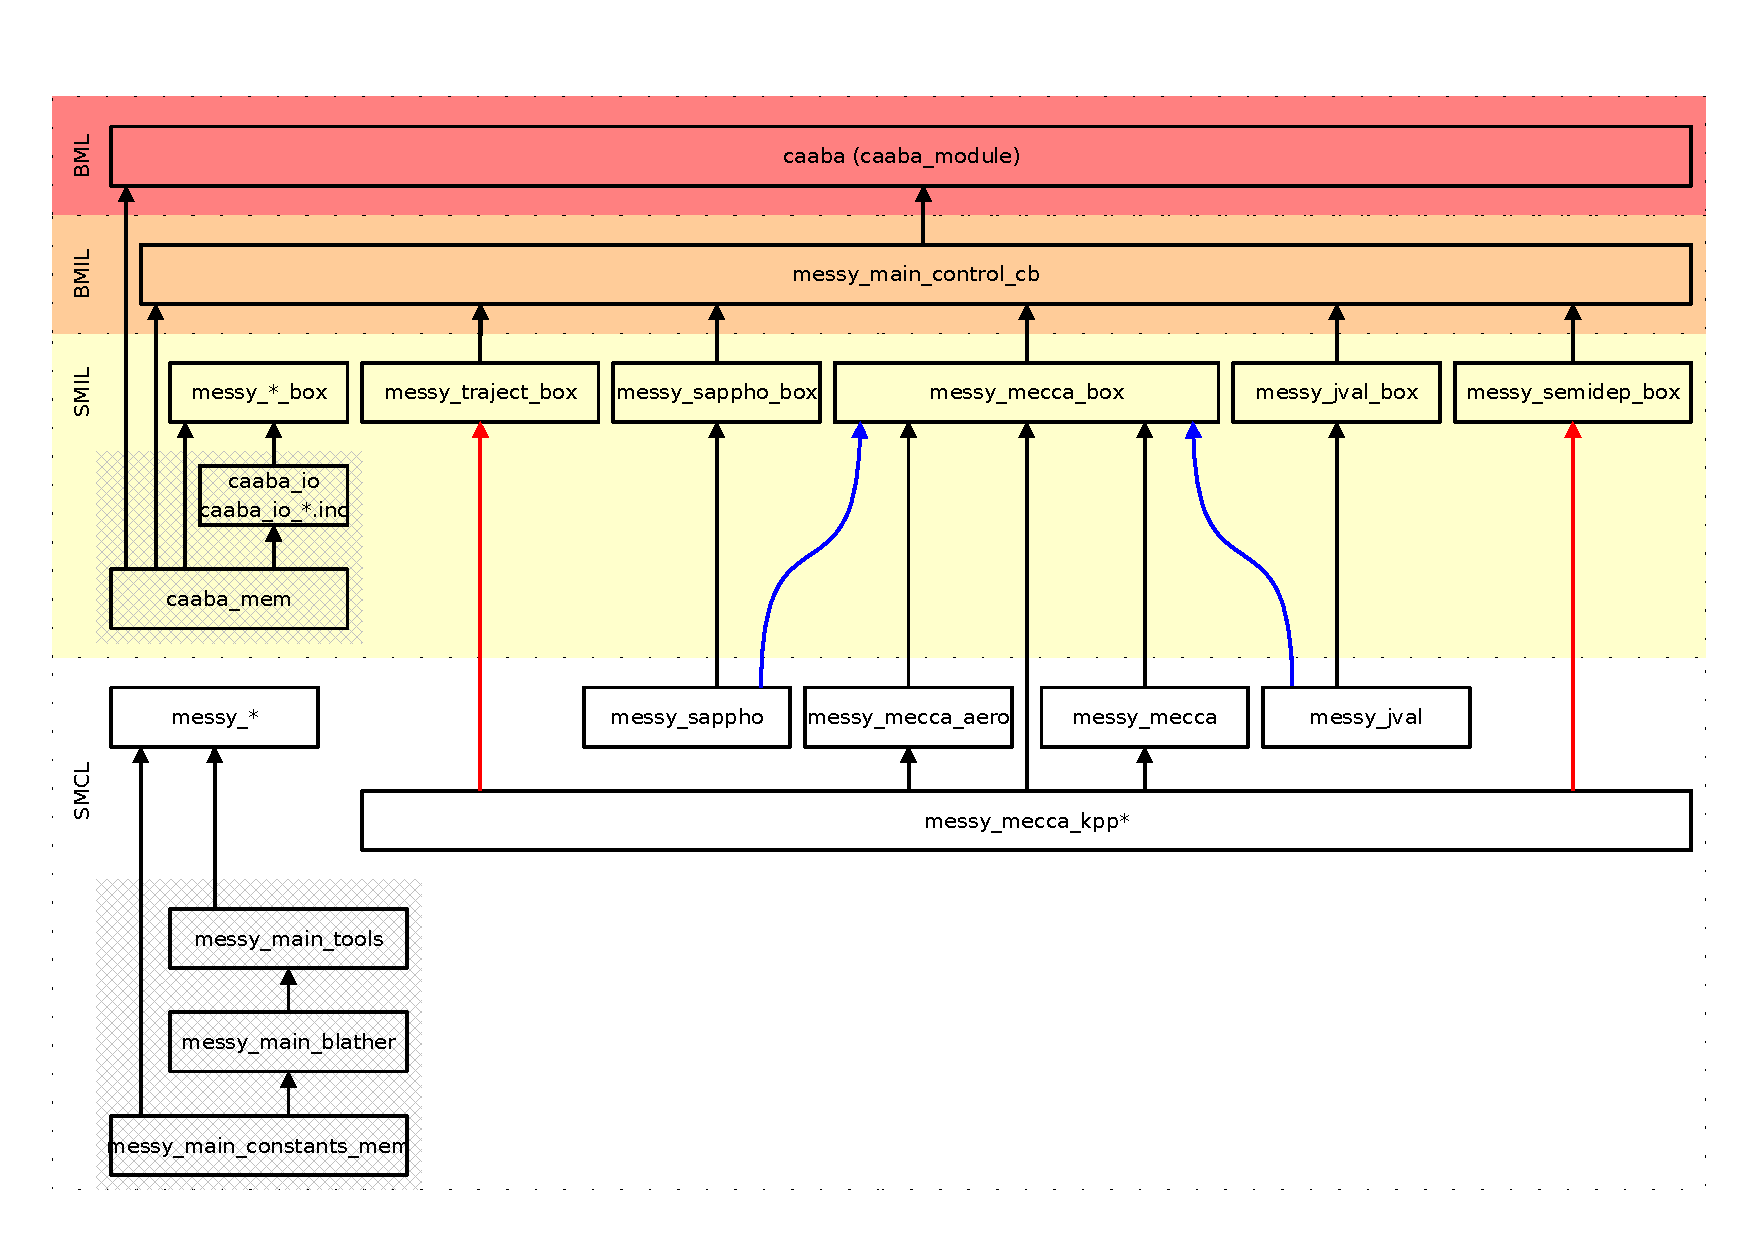
\includegraphics[width=\textwidth]{caaba_use_diagr}
  \end{center}
  \caption{Module structure of MECCA when it is connected to the CAABA
    box model. The box-model related files are in the colored layers
    marked with BML, BMIL, and SMIL. The submodel core layer (SMCL) of
    MECCA is independent of the box model (see \citet{1664} for details
    about the MESSy layers). The arrows start at the module which is
    exporting the variables and subroutines. They point to the module
    importing them via the Fortran90 USE instruction. Here, the box {\tt
      messy\_mecca\_kpp*} represents all KPP-generated files. The
    KPP-internal structure is shown in Fig.~\ref{fig:kpp_use_diagr}.}
  \label{fig:caaba_use_diagr}
\end{figure*}

\begin{figure*}
  \begin{center}
    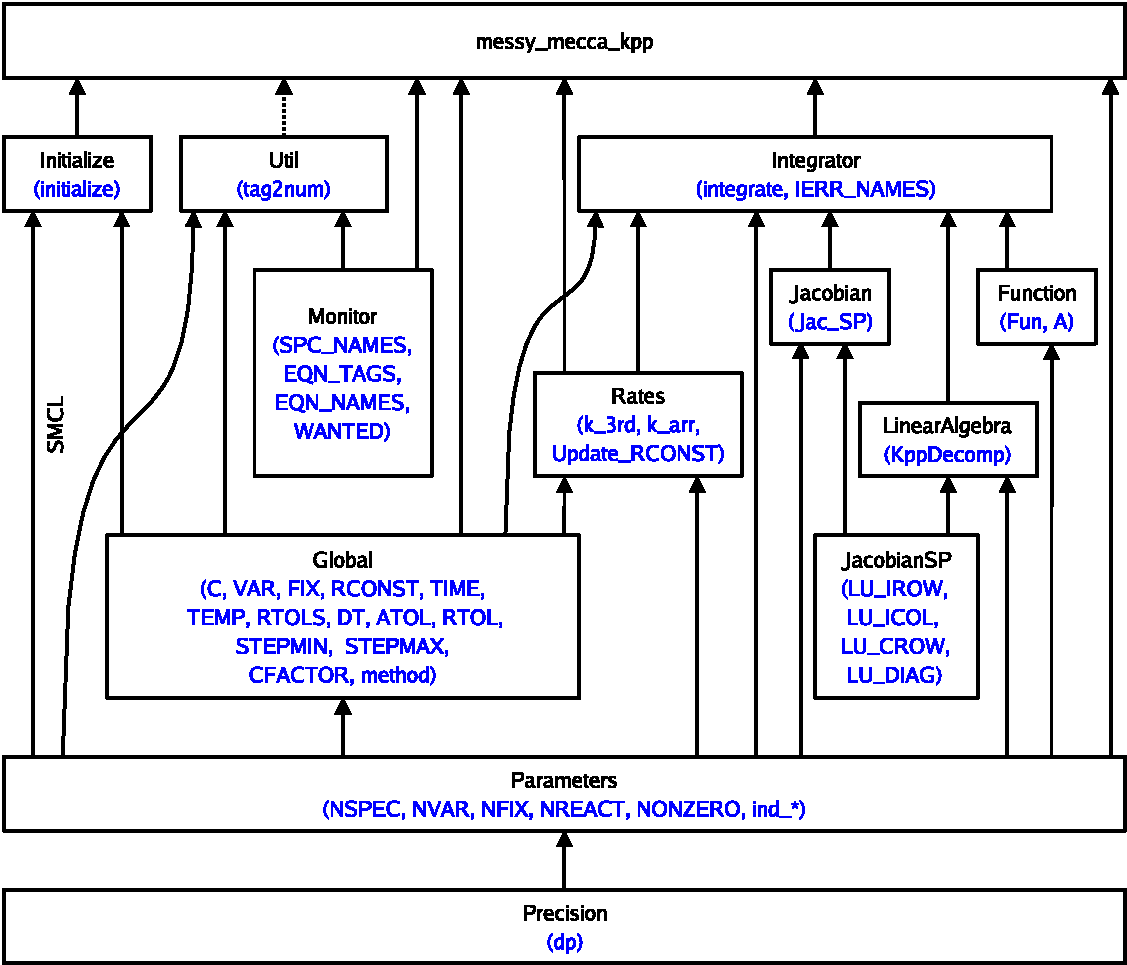
\includegraphics[width=\textwidth]{kpp_use_diagr}
  \end{center}
  \caption{Module structure of KPP-produced Fortran90 files. The arrows
    start at the module which is exporting the variables and subroutines
    shown in blue. They point to the module importing them via the
    Fortran90 USE instruction.}
  \label{fig:kpp_use_diagr}
\end{figure*}

\begin{figure*}
  \begin{center}
    \fbox{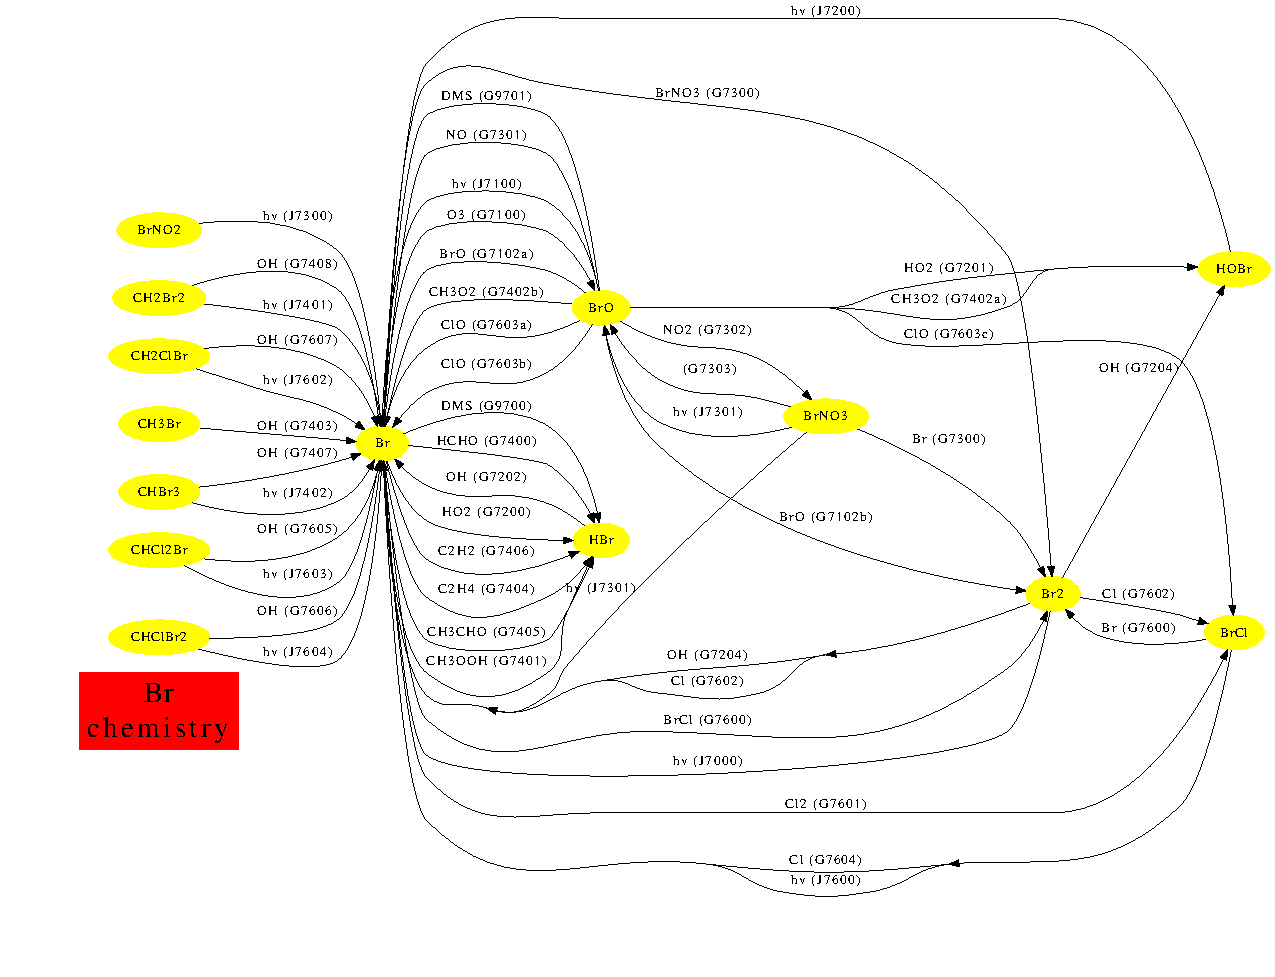
\includegraphics[width=0.9\textwidth]{Br}}
  \end{center}
  \caption{Visualization of the MECCA gas-phase bromine chemistry
    generated with the graphviz software.}
  \label{fig:Br}
\end{figure*}

\subsection{Installation}

Once all prerequisites are fulfilled, you can install CAABA/MECCA by
simply unpacking the zip archive:\\[2mm]
{\tt unzip caaba\_\meccaversion.zip}\\[2mm]

Next, you have to check that all settings in \verb|Makefile| are
correct. If necessary, edit the file: Choose a Fortran90 compiler
(\verb|COMPILER|), enter its name (\verb|F90|) and the compiler options
(\verb|F90FLAGS|). If you add a new compiler, be sure to activate the
C-preprocessor option. To activate netCDF output, you also have to edit
the \verb|Makefile|:
\begin{itemize}\nosep
\item Change the variable \verb|OUTPUT| from \verb|ASCII| to
  \verb|NETCDF|.
\item Enter the correct netCDF library information in
  \verb|NETCDF_INCLUDE| and \verb|NETCDF_LIB|.
\end{itemize}

\subsection{Troubleshooting}

Should there be any problems with the CAABA/MECCA installation, please
check the following:
\begin{itemize}\nosep
\item Confirm that all prerequisites (see above) are fulfilled!
\item Confirm that the perl path in the first line of
  \verb|sfmakedepend| is correct. It should be the same as the output of
  the command:\\
  \verb|which perl|
\item Confirm that the tcsh paths in the first lines of
  \verb|xcaaba| and \verb|xmecca| are correct.
\item Confirm that the model code was unzipped successfully from the zip
  archive. Check for potential problems during the unzipping process:
  \begin{itemize}
  \item Make sure that the directory structure has not changed.
    Unfortunately, some unzipping programs seem to put all files into
    one directory, ignoring the original directory structure.
  \item Make sure that links have not been converted to files. For
    example, the output of the command ``\verb|file caaba.nml|'' should
    tell you that \verb|caaba.nml| is a symbolic link to
    \verb|nml/simple/caaba.nml|.
  \end{itemize}
\end{itemize}

\section{Compiling and running the CAABA/MECCA box model with the shell
  script {\tt xcaaba}}
\label{sec:execute}

First, go to the base directory of the model code (note that all path
names given in this manual are relative to this base directory):\\[2mm]
{\tt cd caaba\_\meccaversion}\\[2mm]
Next, the tcsh script \verb|xcaaba| will guide you through the process
of running the box model. To execute it, type:
\begin{verbatim}
./xcaaba
\end{verbatim}
\verb|xcaaba| will ask several questions, and recommended answers are
given below. If you only press the Return key, you select the default.
\begin{verbatim}
Start xmecca?
\end{verbatim}
If you answer ``y'', you can create a new chemical mechanism with
\verb|xmecca| as described in detail in Sect.~\ref{sec:xmecca}. However,
for the first tests with CAABA/MECCA it is recommended to answer ``n''
and use the simple default mechanism.
\begin{verbatim}
Choose an option:
s = Start from scratch
c = Compile
r = Run existing executable
h = Help
q = Quit
\end{verbatim}
Choose ``c'' to compile the Fortran90 code. After a successful
compilation, \verb|xcaaba| asks if you want to run the model:
\begin{verbatim}
Run CAABA boxmodel with MECCA chemistry?
y = Yes (default)
n = No
m = Multirun (multiple runs)
q = Quit
\end{verbatim}
Answer ``y'' here (see Sect.~\ref{sec:multirun} for more information
about the ``m'' = multirun option).
\begin{verbatim}
Choose a namelist file from
the nml/ directory:
...
\end{verbatim}
Namelists control the behaviour of CAABA/MECCA during run-time, and
editing them allows fine-tuning of the model simulation (see
Sect.~\ref{sec:nmlfiles}). The default is to use the same namelist as
last time. For the first tests, the file \verb|simple/caaba.nml| can be
chosen. Next, \verb|xcaaba| shows the active contents of the namelist
files \verb|caaba.nml| and \verb|mecca.nml|.
\begin{verbatim}
Run CAABA boxmodel with MECCA chemistry?
\end{verbatim}
Answer ``y'', and the CAABA/MECCA model simulation will start. The flow
control is illustrated in Fig:~\ref{fig:caaba_flowcontrol}. The model
day and the current solar zenith angle (sza) are printed on the screen
during the model simulation. The default is to integrate 8 days.
\begin{verbatim}
Save the output and model code 
in output/ directory?
\end{verbatim}
Answer ``y'', and \verb|xcaaba| will put the files into a subdirectory
with a name based on the date and time of the model simulation, e.g.\
\verb|output/2009-08-24-16:29:00/|.

\section{Selecting a chemical mechanism with the shell script {\tt xmecca}}
\label{sec:xmecca}

MECCA contains a very comprehensive set of chemical reactions in both
the gas phase and the aqueous phase. For many applications, using the
complete mechanism will consume too much CPU time. Therefore, the shell
script \verb|xmecca| has been written which allows to create a
custom-made subset of the chemical mechanism interactively. Normally,
\verb|xmecca| is called via \verb|xcaaba|. However, you can also start
it manually:
\begin{verbatim}
cd mecca
./xmecca
\end{verbatim}
\verb|xmecca| will ask several questions, and recommended answers are
given below. If you only press the Return key, you select the default.
\begin{verbatim}
How many aerosol phases?
\end{verbatim}
For a gas-phase only mechanism, type ``0''. For a mechanism with
aqueous-phase chemistry in seasalt and in sulfate particles, type ``2''.
Other values are possible if they have been defined in subroutine
\verb|define_aerosol| in \verb|messy_mecca_box.f90|.
\begin{verbatim}
Modify gas.eqn with a replacement file?
\end{verbatim}
Answer ``0'' unless you have written your own replacement file. More
information about the replacement feature can be found in the file
\verb|rpl/gas.rpl-example|.
\begin{verbatim}
Choose a selection number or type a boolean
expression:
\end{verbatim}
Now you can choose a subset of chemical reactions. A few predefined
standard selections are available. For all other purposes, a batch file
should be created, as explained at the end of this section. Some of the
predefined selections are:
\begin{description}
\item [EVAL:] A mechanism that was used for the evaluation of the MECCA
  chemistry in the global model ECHAM5/MESSy \citep{1851}.
\item [Minimum tropospheric chemistry:] A very small tropospheric
  mechanism.
\item [Minimum MBL chemistry:] A small mechanism that contains
  aqueous-phase chemistry and should only be used if the number of
  aerosol phases is $>0$.
\end{description}
For details about the selection, see Sect.~\ref{sec:selectreactions}.
\begin{verbatim}
Add Monte-Carlo factor to all rate
coefficients? [y/n/q, default=n]
\end{verbatim}
Answer ``n'' here unless you want to perform Monte-Carlo calculations,
as described in Sect.~\ref{sec:montecarlo}.
\begin{verbatim}
Add diagnostic tracers to gas.eqn?
[q/0/?, default=0]
\end{verbatim}
Answer ``0''.
\begin{verbatim}
Calculate accumulated reaction rates
of all equations? [y/n/q, default=n]
\end{verbatim}
Answer ``y'' if you want to have all accumulated reaction rates in the
model output. Otherwise, answer ``n''.
\begin{verbatim}
Tagging, doubling, both, or
none? [t/d/b/n/q, default=n]
\end{verbatim}
Tagging is under construction, so please answer ``n''.
\begin{verbatim}
Run KPP?
\end{verbatim}
Answer ``y''.
\begin{verbatim}
Choose an integrator [q=quit,
default=rosenbrock_posdef]:
\end{verbatim}
The default integrator is strongly recommended (see
Sect.\ref{sec:selectintegrator} for details). Next, KPP will create
several Fortran90 files.
\begin{verbatim}
Remove indirect indexing with decomp?
[y/n/q, default=n]
\end{verbatim}
If this question shows up, answer ``n''.
\begin{verbatim}
Create LaTeX listing of selected mechanism?
[y/n/q, default=n]
\end{verbatim}
If you answer ``y'' here, a table of the current reaction mechanism will
be produced. Only the selected reactions will be listed. The table also
contains the rate coefficients and their references, as described in
Sect.~\ref{sec:latextable}.
\begin{verbatim}
Create graphviz plots of selected
mechanism? [y/n/q, default=n]
\end{verbatim}
If you have the ``\verb|dot|'' program from the graphviz software
installed, you can create graphical visualizations of the reaction
mechanism. As an example, the graphviz-generated plot of gas-phase
bromine chemistry is shown in Fig.~\ref{fig:Br}. For more information,
look at the files \verb|xgraphvizall|, \verb|xgraphviz|, and
\verb|spc_extract.awk| in the \verb|mecca/graphviz/| directory.
\begin{verbatim}
Do you want to delete the temporary
xmecca files?
\end{verbatim}
It is okay to delete these temporary files unless you need them for
debugging purposes.

When \verb|xmecca| finishes successfully, the Fortran90 code of your
selected mechanism has been created. The KPP-produced Fortran90 files
(Tab.~\ref{tab:files}) are moved into the \verb|mecca/smcl/| directory
(with lower-case names). An exception is
\verb|messy_mecca_kpp_Model.f90|, which is produced by KPP but not
needed for MECCA. The modular structure of the KPP-produced Fortran90
files is shown in Fig.~\ref{fig:kpp_use_diagr}.

If you need to create a chemical mechanism very often, it is quite
tedious to answer all questions every time. To make this easier, you can
copy the template \verb|batch/example.bat| to a new name (e.g.\
\verb|batch/myfile.bat|) and then enter your answers into that batch
file. Now you can create a new chemical mechanism in batch mode with
\begin{verbatim}
./xmecca myfile
\end{verbatim}
It is also possible to add the name of the batch file to the
\verb|xcaaba| command:
\begin{verbatim}
./xcaaba myfile
\end{verbatim}

\subsection{Selecting a set of chemical reactions}
\label{sec:selectreactions}

All chemical reactions are marked. Each marker consists of several
labels which contain information about the altitude
(troposphere/stratosphere), the phase where the reaction occurs
(gas/aqueous), its relevant chemical elements, and more. See
Sect.~\ref{sec:markerslabels} for a complete list of labels. To define a
set of chemical reactions, you can either choose a pre-defined selection
by number or enter a boolean expression based on the labels. Boolean
expressions are typed in awk syntax. The most important operators and
expressions are:\\
\begin{tabular}{l@{ = }l}
\verb|&&| & AND\\
\verb!||! & OR\\
\verb|!|  & NOT\\
\verb|()| & parentheses\\
\verb|1|  & TRUE\\
\verb|0|  & FALSE
\end{tabular}

For example, to select all gas-phase reactions (G) except for those
including halogens (Cl, Br, I), type:

\verb|G && !Cl && !Br && !I|.

It is important to understand the logic behind this selection mechanism.
The expression ``\verb|Cl && Br|'' selects only those reactions that
contain chlorine {\em and} bromine. Similarly, the expression
``\verb|G && Het|'' selects only those reactions that occur in the gas
phase {\em and} and are heterogeneous. However, since no reaction has
both the ``\verb|G|'' {\em and} the ``\verb|Het|'' label, this results
in an empty mechanism. If you want a mechanism that contains both
gas-phase and heterogeneous reactions, you must select all reactions
that contain either the label ``\verb|G|'' {\em or} the label
``\verb|Het|'', i.e.\ you must use the expression ``\verb!G || Het!''.

\subsection{Selecting a numerical integrator}
\label{sec:selectintegrator}

Several numerical integrators are defined in the subdirectory
\verb|mecca/kpp/int/| and can be used with KPP. The default is the
positive definite Rosenbrock solver with automatic time-step control
(\verb|rosenbrock_posdef|). It is very robust and capable of integrating
very stiff sets of equations (e.g.\ chemical mechanisms including both
gas- and aqueous-phase chemistry). Although a Rosenbrock solver with
manual time-step control (\verb|ros2_manual|) is also available, it is
strongly recommended not to use it for stiff sets of equations. If you
choose it, you do so at your own risk!

\section{Plotting the model results with the ferret software}
\label{sec:ferret}

If you have chosen netCDF output, you can plot the model results with
the ferret program (\url{http://ferret.wrc.noaa.gov/Ferret/}). Change
into the \verb|jnl/| directory, then start the program by typing
``\verb|ferret|''. When ferret has started, you can plot the gas-phase
species of the latest model simulation with the ferret script
\verb|xxxg.jnl| by typing:
\begin{verbatim}
go xxxg.jnl
\end{verbatim}
Similarly, \verb|xxxa.jnl| can be used to plot aqueous-phase species:
\begin{verbatim}
go xxxa.jnl
\end{verbatim}
The file \verb|xxxa.jnl| accepts several parameters to modify the plots.
The first parameter should be ``\verb|0d|'' for plotting box model
results. The second parameter can be set to ``\verb|mpl|'' or
``\verb|mpm|'' in order to plot either aqueous-phase concentrations
[\unit{mol/L}] or mixing ratios [\unit{mol(aq)/mol(air)}], respectively.
The third parameter defines the aerosol bin. With two aerosol bins,
``\verb|A01|'' refers to sulfate particles, and ``\verb|A02|'' to
sea-salt particles. For example, type:
\begin{verbatim}
go xxxa.jnl 0d mpl A02
\end{verbatim}
Photolysis rate coefficients can be plotted with \verb|jval.jnl|:
\begin{verbatim}
go jval.jnl
\end{verbatim}
If the calculation of accumulated reaction rates had been switched on in
\verb|xmecca| (see Sect.~~\ref{sec:xmecca}), plots of the reaction rates
can be made. One possibility is to plot all reactions with:
\begin{verbatim}
go rxnrates.jnl
\end{verbatim}
Alternatively, it is possible to plot only the production and
destruction rates for a certain species, e.g.\ for OH:
\begin{verbatim}
go rxnrates_scaled.jnl OH
\end{verbatim}
To plot results from previous simulations which are saved in the
\verb|output/| directory, edit the file \verb|setmodelrun.jnl| and enter
the paths of the directories in the ``\verb|GO _define_sensi|'' command.
To compare model simulations, you can enter two or more
``\verb|GO _define_sensi|'' commands in \verb|setmodelrun.jnl|. To plot
the difference between model simulations, activate the line
``\verb|DEFINE SYMBOL diffplot TRUE|'' in \verb|setmodelrun.jnl|.

\section{Run CAABA/MECCA in special modes}
\label{sec:special}

In the base configuration described so far, CAABA/MECCA calculates the
temporal evolution of the chemistry inside an air parcel. This is ideal
for sensitivity studies analyzing the effect of individual reactions
inside a large chemical mechanism. For other applications, some special
modes exist as described below.

\subsection{Multiple model simulations and steady-state}
\label{sec:multirun}

The so-called ``multirun'' mode performs multiple model simulations,
each of them terminating when a steady-state has been reached. This is
useful to calculate the steady-state concentrations of short-lived
species (e.g.\ OH) when the concentrations of longer-lived species
(e.g.\ non-methane hydrocarbons) are known from measurements. The
default termination condition is that the change of OH between two model
time steps is less than 0.1~\unit{\%}. If necessary, this can be changed
in the function \verb|steady_state_reached| in \verb|messy_mecca.f90|.
To avoid that the concentrations of long-lived species change from their
initial values, they can be fixed in the file
\verb|mecca/messy_mecca_kpp.kpp| by adding them to the
``\verb|#SETFIX|'' line. Initial mixing ratios and J-values must be
available in netCDF files in the \verb|multirun/input/| directory. As an
example, the file \verb|example.nc| is available. To create such input
netCDF files from ASCII files, the script \verb|asc2ferret4nc.tcsh| can
be used. Finally, since the multirun mode needs ``\verb|ncks|'' from the
netCDF Operators (NCO) software, it must be ensured that this program is
available. After these preparations, the multirun mode can be entered by
running \verb|xcaaba| and answering the question ``Run CAABA boxmodel
with MECCA chemistry?'' with ``m''. This will start the
\verb|multirun.tcsh| script in the \verb|multirun/| directory. The user
can either select one input file or make model simulations for all input
files in the \verb|multirun/input/| directory. For each input netCDF
file, the script \verb|loopcaaba.tcsh| is called. For each time step
contained in the input file, \verb|loopcaaba.tcsh| performs a
CAABA/MECCA model simulation. It first creates a suitable namelist file
\verb|caaba.nml|. Values for temperature and pressure are transferred
from the input netCDF file to the namelist file. In addition,
\verb|loopcaaba.tcsh| creates two important settings in
\verb|caaba.nml|: First, the steady-state option is switched on with
``\verb|l_steady_state_stop = T|''. Second, the submodel READJ is
activated and used with ``\verb|USE_READJ = T|'' and
``\verb|photrat_channel = 'readj'|''. After the model simulations have
finished, a summary of the output is placed in the output directory. The
name of the output directory will be based on the name of the input
netCDF file, e.g.\ when the file \verb|example.nc| is used, the output
will be in \verb|output/multirun/example/|.

\subsection{Monte-Carlo}
\label{sec:montecarlo}

\subsubsection{Performing Monte-Carlo simulations}

In the Monte-Carlo mode, several CAABA/MECCA simulations are performed,
with each individual simulation using slightly different rate
coefficients. To activate it, you first have to create a new chemistry
mechanism with \verb|xmecca| (see Sect.~\ref{sec:xmecca}) and answer the
question ``Add Monte-Carlo factor to all rate coefficients'' with ``y''.
This will start the awk script \verb|mcfct.awk|, which adds Monte-Carlo
factors to the rate coefficients in the equation file. Next, the
\verb|xcaaba| script can be used to start the simulations. It will start
the script \verb|montecarlo.tcsh| in the directory \verb|montecarlo/|.
The default is to make 5 model simulations. To choose another value (up
to 9999), change the definition of \verb|maxline| in
\verb|montecarlo.tcsh|.

\subsubsection{Analyzing Monte-Carlo simulations}

After performing the model simulations, the resulting netCDF files are
merged (using the tools \verb|ncpdq|, \verb|ncclamp|, and \verb|ncrcat|)
and then stored in the output directory with a name based on the date
and time of the model simulations, e.g.\ \verb|$outputdir| =
\verb|output/montecarlo/2010-06-24-16:29:00|. The final concentrations
and rate coefficients of all simulations are summarized in
\verb|caaba_mecca_c_end.nc| and \verb|caaba_mecca_k_end.nc|. Results of
the individual simulations can be found in the directories
\verb|$outputdir/runs/*|.

\paragraph{Time series}

If the model is set up to run for a fixed length (e.g.\ using the
default of \verb|ext_runtime| = 8 days), the time series of all
simulations can be plotted together with ferret by activating the lines
for Monte-Carlo in \verb|setmodelrun.jnl|. However, these plots become
illegible if more than about 5 simulations are made.

\paragraph{Steady-state calculations}

The most efficient way to analyze a large number of Monte-Carlo
simulations is to use the steady-state option and only compare the
final values of the different model simulations, not the individual time
series. The ferret script \verb|montecarlo.jnl| can be used to create
scatter plots of concentrations vs rate coefficients. It also plots
linear regression lines for all comparisons above a certain threshold of
the correlation coefficient (default: $r^2>0.05$).

\subsubsection{Variation of rate coefficients}

In each individual Monte-Carlo simulation $j$, all rate coefficients
$k_i$ are varied by a Monte-Carlo factor:

\begin{equation}
  k^{\rm MC}_{i,j} = k_i \times f_i^{x_{i,j}}
\end{equation}

Here, $k^{\rm MC}_{i,j}$ is the rate coefficient of reaction $i$ used in
the Monte-Carlo simulation $j$. It is defined as the product of the
recommended value $k_i$ and the Monte-Carlo factor $f_i^{x_{i,j}}$. This
Monte-Carlo factor consists of two parts, the uncertainty factor $f_i$
and the exponent $x_{i,j}$:

\paragraph{The uncertainty factor $f_i$} 

The uncertainty factor $f_i$ describes the uncertainty of the measured
(or estimated) rate coefficient $k_i$. Its value can usually be found in
publications of laboratory studies or summaries like the JPL evaluation
\citep{1945}.

The tables of the IUPAC evaluations \egcite{1759} list the decadic
logarithm $\lg(f_i)$ of the uncertainty factor, which they call
``$\Delta\log k$''.

Sometimes an absolute uncertainty is quoted instead of an uncertainty
factor, e.g.\ $k = 2 \pm 0.2$ or $k = 2 \pm 10\%$. In this case we
define $f_i$ such that the upper limit is reached when multiplied with
$k_i$, i.e.\ in the current example $f_i = (2+0.2)/2 = 1.1$.

The uncertainty factor is defined in the equation files (\verb|*.eqn|)
in a comment starting with the paragraph symbol. Three different syntax
types are possible:
\begin{itemize}
\item If there is just one \verb|§| sign, (e.g.\ ``\verb|{§1.1}|''), the
  value inside the curly braces is the uncertainty factor $f_i$.
\item With two \verb|§| signs, (e.g.\ ``\verb|{§§0.04}|''), the value
  inside the curly braces equals $\lg(f_i)$.
\item If there is only a \verb|§| sign (``\verb|{§}|'') but no number,
  the uncertainty factor is set to the default value of $f_i$~= 1.25.
\end{itemize}

\paragraph{The Monte-Carlo exponent $x_{i,j}$} 

There is one Monte-Carlo exponent $x_{i,j}$ (variable ``\verb|mcexp|''
in the code) for each rate coefficient $k_i$ and for each individual
Monte-Carlo simulation $j$. The values of $x_{i,j}$ are
normally-distributed random numbers centered around zero, and produced
with the Marsaglia polar method
(\url{http://en.wikipedia.org/wiki/Marsaglia_polar_method}). As input
for the Marsaglia polar method, uniformly distributed random numbers
between 0 and 1 calculated with either the standard Fortran90 function
{\tt RANDOM\_NUMBER} or the Mersenne Twister algorithm \citep{2404} are
used.

\subsubsection{Changing the uncertainty factors}

The uncertainty factors can be changed by modifying the equation files,
as shown in Sect.~\ref{sec:eqnfiles}. Note that predefined rate
coefficients (e.g.\ \verb|k_HO2_HO2|) already contain an uncertainty
factor and there must not be an additional factor in the reaction where
they are used.

In some cases, it may be useful to vary only one or a few rate
coefficients. To do this, it is first necessary to find the correct
indices of \verb|mcexp(...)| in \verb|mecca.eqn| (note that these
indices may change when creating a new mechanism with \verb|xmecca|). As
an example, to vary only the rate coefficients that use \verb|mcexp(40)|
and \verb|mcexp(50)|, the following lines can be added to subroutine
\verb|mecca_init| in \verb|messy_mecca_box.f90| after
\verb|CALL define_mcexp|:
\begin{verbatim}
DO i=1, MAX_MCEXP
  IF ((i/=40).OR.(i/=50)) mcexp(i) = 0.
ENDDO
\end{verbatim}

To verify that the rate coefficients are modified in the Monte-Carlo
simulations, it is possible to temporarily activate the subroutine
\verb|montecarlo_check| in \verb|template_messy_mecca_kpp.f90| and check
the output in \verb|caaba.log|. After these tests,
\verb|montecarlo_check| must be switched off again to allow normal model
simulations.

\subsection{Lagrangian trajectories}
\label{sec:lagrangian}

CAABA can be used as a Lagrangian trajectory box model \citep{2403}. The
usual combination of submodels for this purpose includes the CAABA
submodel TRAJECT for the processing of trajectory information, MECCA for
atmospheric chemistry, and JVAL for photolysis rate calculation. All
important settings for trajectory calculations can be made via the
namelist file plus a few external files.

\subsubsection{Namelist parameters}

A namelist template can be found in
\verb|nml/caaba_traject_example.nml|. After copying the namelist file to
a new name in the same directory and altering the settings, it will be
available when running caaba via \verb|xcaaba|. There are standard and
trajectory-exclusive namelist parameters to be set:
\begin{itemize}\nosep
\item \noindent\textbf{Submodel switches (mandatory):} The trajectory
  mode of CAABA requires that \verb|USE_TRAJECT = T|,
  \verb|USE_MECCA = T|, and \verb|USE_JVAL = T| and/or
  \verb|USE_SAPPHO = T|. One of the two photolysis rate models is
  sufficient, but it is also possible to run them in parallel (see also
  \verb|photrat_channel|). If the use of external photolysis rates is
  desired, \verb|USE_JVAL = T| is mandatory. For the application in
  \citet{2403}, the submodel \verb|SEMIDEP| was switched off.
  (\verb|!USE_SEMIDEP = T|).
\item \textbf{Scenarios (optional):} Scenarios may be used in trajectory
  mode. When using external input for chemical initialization and
  photolysis rates, however, they can be ignored (commented out, e.g.,
  \verb|!init_scenario = ''|) or used as complement.
\item \textbf{Photolysis rate channel:} Choose
  \verb|photrat_channel = 'jval'| when planning to prescribe photolysis
  rates.
\item \textbf{Trajectory input (mandatory):} The path to the netCDF file
  containing trajectory waypoints should be specified as
  \verb|input_physc = 'traject/example_traj.nc'|. For its structure, see
  section \ref{sec:trajfile}.
\item \textbf{Tracer initialization (optional):} Tracer mixing ratios
  can be initialized with an external netCDF file by specifying the path
  to it with \verb|init_spec = 'traject/example_init.nc'|. For its
  structure, please refer to section \ref{sec:tracfile}.
\item \textbf{Photolysis rates (optional):} For prescribed photolysis
  rates, specify the path to the respective file as
  \verb|input_jval = 'traject/example_jval.nc'|. For its structure, see
  \ref{sec:jvalfile}.
\item \textbf{Variable names (partly mandatory):} There are default
  trajectory variable names designated in CAABA. They can be selectively
  changed by providing alternative variable names. Here is a list of
  trajectory variables, their default name, and respective examples how
  to specify an alternative variable name:
  \begin{center}
    \begin{tabular}{lll}
      \hline
      quantity       & default      & alternative\\
      \hline
      longitude      & \verb|LON|   & \verb|vlon = 'LON_TR'|\\    
      latitude       & \verb|LAT|   & \verb|vlat = 'LAT_TR'|\\
      pressure       & \verb|PRESS| & \verb|vpress = 'P'|\\
      temperature    & \verb|TEMP|  & \verb|vtemp = 'TM1'|\\
      rel. humidity  &              & \verb|vrelhum = 'rh'|\\
      spec. humidity &              & \verb|vspechum = 'sh'|\\
      \hline
    \end{tabular}
  \end{center}
  Humidity has no default variable name due to the choice of either
  providing relative humidity or specific humidity. Thus, it is
  mandatory to specify exactly one of the two in the namelist. When
  specific humidity is provided, then both specific humidity and
  relative humidity are written to the output \verb|caaba_physc.nc|,
  since CAABA uses relative humidity internally. When relative humidity
  is provided, only relative humidity will be written to output.
\item \textbf{Integration time (optional):} \verb|time_step| sets the
  integration and output time step. See also section
  \ref{sec:caaba_nml}.
\item \textbf{Clipping the trajectory (optional):} Two namelist
  parameters allow flexible cropping of the model runtime along the
  trajectory. \verb|runlast| defines the start of the CAABA simulation
  counted backwards in time from the trajectory end, i.e.
  \verb|runlast = 4.5| means ``calculate the last 4.5 days of the
  trajectory''. The unit is days. The parameter \verb|ext_runtime|
  defines the overall model simulation time. Thus, \verb|runlast| and
  \verb|ext_runtime| combined clip out any desired part of the
  trajectory.
\end{itemize}

\subsubsection{Trajectory input file}
\label{sec:trajfile}

The trajectory information is provided to CAABA via an external netCDF
file specified in the namelist by \verb|input_physc|. A sample file is
available at \verb|traject/example_traj.nc|. The file should contain a
time origin in 'seconds/minutes/hours/days since yyyy-mm-dd hh:mm:ss',
where the seconds in the time string are optional, for example:
\verb|"MINUTES since 2000-01-19 08:00:00"|. The file must contain at
least two trajectory waypoints and the following time-dependent
variables:

\begin{center}
  \begin{tabular}{lll}
    \hline
    quantity       & default name &  unit\\
    \hline
    longitude      & \verb|LON|   &  degrees east\\
    latitude       & \verb|LAT|   &  degrees north\\
    pressure       & \verb|PRESS| &  Pascal\\
    temperature    & \verb|TEMP|  &  Kelvin\\
    (rel. humidity)  &            &  1\\
    (spec. humidity) &            &  kg/kg\\
    \hline
  \end{tabular}
\end{center}

Of the two humidity quantities, only one needs to be present.

\subsubsection{Photolysis rate file}
\label{sec:jvalfile}

It is possible to prescribe photolysis rate coefficients via netCDF
file. An example is available at \verb|traject/example_jval.nc|. At the
moment, only photolysis rates for the species \chem{NO_2} can be read
into the model and must have the variable name \verb|J_NO2|. The files
specified in \verb|input_jval| (e.g.\ \verb|example_jval.nc|) and
\verb|input_physc| (e.g.\ \verb|example_traj.nc|) must both refer to
exactly the same trajectory as the photolysis rate values are read into
the model at the same times as other trajectory information.

\subsubsection{Tracer initialization file}
\label{sec:tracfile}

There are default initial values included in MECCA for a variety of
species and simulation aims (see \verb|init_scenario|). However, for
several consecutive simulations with changing initialization, the
possibility to define an initialization file using \verb|init_spec| is
convenient. The tracer initialization file is a netCDF file with one
point in time, at which selected species' mixing ratios are defined in
mol/mol. The point in time itself is not important and not checked when
reading the initial mixing ratios. All tracers that are not specified in
\verb|init_spec| are initialized according to default or a chosen
\verb|init_scenario|. An example for the initialization file can be
found at \verb|traject/example_init.nc|.

\subsubsection{Trajectory mode output}

Output along the trajectory is written to \verb|caaba_messy.nc|. There
are some special variables written out in addition to the default
\verb|caaba_messy.nc| output. They are listed in the second part of the
table.

\begin{tabular}{lll}
  \hline
  variable         & unit             & notes\\
  \hline
  \verb|lon|       & \multicolumn{2}{l}{(dummy 3-D x-coordinate)}\\
  \verb|lat|       & \multicolumn{2}{l}{(dummy 3-D y-coordinate)}\\
  \verb|lev|       & \multicolumn{2}{l}{(dummy 3-D z-coordinate)}\\
  \verb|time|      & \textless unit\textgreater  since ... & time\\
  \verb|lon_tr|    & deg east         & longitude\\
  \verb|lat_tr|    & deg north        & latitude\\
  \verb|press|     & Pa               & pressure\\
  \verb|temp|      & K                & temperature\\
  \verb|relhum|    & 1                & relative humidity (RH)\\
  \hline
  \verb|spechum|   & kg/kg            & specific humidity ($q$)\\
  \verb|sza|       & deg              & solar zenith angle\\
  \verb|J_NO2_x|   & 1/s              & \chem{NO_2} photolysis rate\\
  \verb|localtime| & same as time     & local time\\
  \verb|year_loc|  &                  & year of local time\\
  \verb|month_loc| &                  & month of local time\\
  \verb|day_loc|   &                  & day of local time\\
  \verb|hour_loc|  &                  & hour of local time\\
  \verb|min_loc|   &                  & minute of local time\\
  \verb|sec_loc|   &                  & second of local time\\
  \hline
\end{tabular}

The specific humidity $q$ is only written to output if it was provided
as input. In that case, the relative humidity RH is calculated using the
WMO definition \citep{1660}:
\begin{equation}
  \mbox{RH} = \frac{\omega_v}{\omega_{vs}} = 
\frac{p_{\chem{H_2O}}(T)}{p - p_{\chem{H_2O}}(T)} \times
\frac{p - p_{\rm sat}(T)}{p_{\rm sat}(T)}
\end{equation}
with $\omega_v$~= water vapor mass mixing ratio and $\omega_{vs}$~=
saturation water vapor mass mixing ratio. We calculate these as:
\begin{eqnarray}
  \omega_v & = & \frac{q}{1-q}\\
  \omega_{vs} & = & \frac{M(\chem{H_2O})}{M({\rm air})} \times
  \frac{p_{\rm sat}(T)}{p - p_{\rm sat}(T)} 
\end{eqnarray}
using the pressure $p$, the temperature-dependent saturation water vapor
pressure $p_{\rm sat}(T)$, and the molar masses $M$ of water and dry
air.

\begin{table*}%[htb]
  \begin{center}
    \caption{List of CAABA/MECCA Fortran90 files}
    \label{tab:files}
    \begin{tabular}{lp{0.55\textwidth}}
      \hline
      \multicolumn{2}{l}{CAABA box model related files}\\
      \hline
      \verb|caaba.f90|                         & main box model file\\
      \verb|caaba_io.f90|                      & input/output\\
      \verb|caaba_io_netcdf.inc|               & netCDF input/output\\
      \verb|caaba_io_ascii.inc|                & ASCII input/output\\
      \verb|caaba_mem.f90|                     & declaration of CAABA variables\\
      \verb|messy_main_control_cb.f90|         & flow control\\
      %\verb|messy_e4chem_box.f90|              & connection of E4CHEM to CAABA\\
      \verb|messy_jval_box.f90|                & connection of JVAL to CAABA\\
      \verb|messy_mecca_box.f90|               & connection of MECCA to CAABA\\
      \verb|messy_mecca_dbl_box.f90|           & (under construction)\\
      \verb|messy_mecca_tag_box.f90|           & (under construction)\\
      \verb|messy_readj_box.f90|               & connection of READJ to CAABA\\
      \verb|messy_sappho_box.f90|              & connection of SAPPHO to CAABA\\
      \verb|messy_semidep_box.f90|             & simplified emission and
                                                 deposition, including
                                                 connection to CAABA\\
      \verb|messy_traject_box.f90|             & trajectory calculations\\
      % \hline
      % \multicolumn{2}{l}{ECHAM5 related files}\\
      % \hline
      % \verb|messy_mecca_e5.f90|                & interface between ECHAM5 and
      %                                            MECCA subroutines\\
      % \verb|messy_mecca_aero_e5.f90|           & interface between ECHAM5 and
      % MECCA-AERO subroutines\\
      % \verb|messy_mecca_mem_e5.f90|            & declaration and
      %                                            memory for variables\\ 
      % \verb|messy_mecca_idt_e5.inc|            & include file\\
      % \verb|messy_mecca_c2mr_e5.inc|           & include file\\
      % \verb|messy_mecca_mr2c_e5.inc|           & include file\\
      % \verb|messy_mecca_trac_e5.inc|           & include file\\
      % \verb|mecca_t.nml|                       & namelist for tracer
      %                                            initialization\\
      \hline
      \multicolumn{2}{l}{static core files}\\
      \hline
      \verb|messy_cmn_photol_mem.f90|          & common definitions for photolysis\\
      \verb|messy_main_constants_mem.f90|      & physical constants\\
      \verb|messy_main_blather.f90|            & print utilities\\
      \verb|messy_main_rnd.f90|                & random number generation\\
      \verb|messy_main_rnd_lux.f90|            & Luxury random numbers\\
      \verb|messy_main_rnd_mtw.f90|            & Mersenne-Twister random numbers\\
      \verb|messy_main_timer.f90|              & timer\\
      \verb|messy_main_tools.f90|              & auxiliary functions\\
      \verb|messy_main_tools_kp4_compress.f90| & (file exists but is not
                                                 not used with CAABA)\\
      %\verb|messy_e4chem.f90|                  & \\
      \verb|messy_jval.f90|                    & calculation of J-values\\
      \verb|messy_jval_jvpp.inc|               & include file for JVAL\\
      \verb|messy_readj.f90|                   & read J-values\\
      \verb|messy_sappho.f90|                  & simplified and parameterized 
                                                 photolysis rate coefficients\\
      \hline
      \multicolumn{2}{l}{static MECCA core files in the {\tt mecca/smcl/}
        directory}\\
      \hline
      \verb|messy_mecca.f90|                   & MECCA core\\
      \verb|messy_mecca_aero.f90|              & aerosol chemistry\\
      \verb|messy_mecca_khet.f90|              & (file exists but is not
                                                 used with CAABA)\\
      \hline
      \multicolumn{2}{l}{KPP- and {\tt xmecca}-produced files in the {\tt
          mecca/smcl/} directory}\\
      \hline
      \verb|messy_mecca_kpp.f90|               & a wrapper for the KPP files\\
      \verb|messy_mecca_kpp_function.f90|      & ODE function\\
      \verb|messy_mecca_kpp_global.f90|        & global data headers\\
      \verb|messy_mecca_kpp_initialize.f90|    & initialization\\
      \verb|messy_mecca_kpp_integrator.f90|    & numerical integration\\
      \verb|messy_mecca_kpp_jacobian.f90|      & ODE Jacobian\\
      \verb|messy_mecca_kpp_jacobiansp.f90|    & Jacobian sparsity\\
      \verb|messy_mecca_kpp_linearalgebra.f90| & sparse linear algebra\\
      \verb|messy_mecca_kpp_monitor.f90|       & equation info\\
      \verb|messy_mecca_kpp_parameters.f90|    & model parameters\\
      \verb|messy_mecca_kpp_precision.f90|     & arithmetic precision\\
      \verb|messy_mecca_kpp_rates.f90|         & user-defined rate laws\\
      \verb|messy_mecca_kpp_util.f90|          & utility input-output\\
      \hline
    \end{tabular}
  \end{center}
\end{table*}

\section{Modifying CAABA/MECCA}
\label{sec:modifying}

\begin{figure*}%[htb]
  \begin{center}
  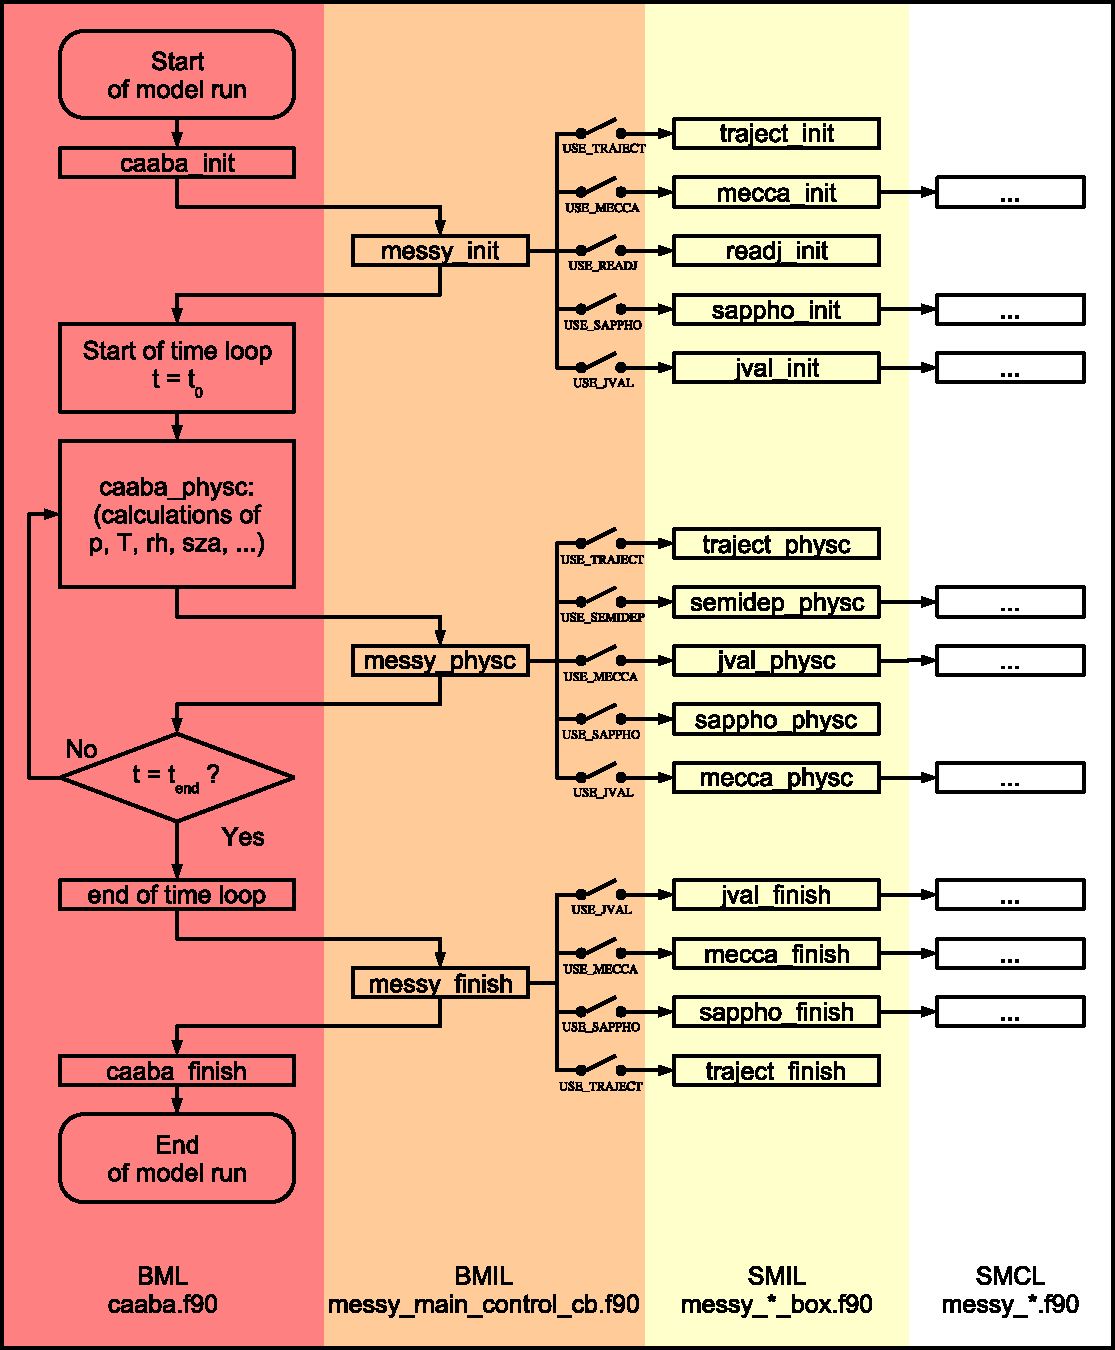
\includegraphics[width=\textwidth]{caaba_flowcontrol}
  \end{center}
  \caption{Flow control of a CAABA box model simulation}
  \label{fig:caaba_flowcontrol}
\end{figure*}

The CAABA/MECCA model simulation can be modified by changing the
namelist files (\verb|*.nml|), the species files (\verb|*.spc|), the
equation files (\verb|*.eqn|) and the Fortran90 files (\verb|*.f90|).

\subsection{Namelist files}
\label{sec:nmlfiles}

Fortran90 namelist files allow modifications of the model simulation
without having to recompile the source code.

\subsubsection{The CAABA namelist file {\tt caaba.nml}}
\label{sec:caaba_nml}

The file \verb|caaba.nml| contains the namelist \verb|&CAABA|. Here
individual parts of the CAABA model (the so-called ``MESSy submodels'')
can be switched on or off. It is important that the following switches
are set to ``T'' (=true):
\begin{verbatim}
USE_MECCA   = T
USE_SAPPHO  = T
USE_SEMIDEP = T
\end{verbatim}
To use the photolysis rate coefficients from SAPPHO in MECCA, set:
\begin{verbatim}
photrat_channel = 'sappho'
\end{verbatim}
Alternatively, you can switch on the JVAL submodel with
\verb|USE_JVAL = T| and then select \verb|photrat_channel = 'jval'|. It
is fine to switch on both the JVAL and the SAPPHO submodel, which can be
useful for a comparison. However, only the values selected by
\verb|photrat_channel| are used for the MECCA chemistry.

You can define the model start, runtime, and time step, e.g.:
\begin{verbatim}
startday    = 90.
ext_runtime = '10 days'
time_step   = '15 minutes'
\end{verbatim}
If you don't set these, the default is a model start on Julian day 80, a
model simulation duration of 8 days, and an output time step of 20
minutes. The \verb|time_step| value can be given as any integer or
floating point and in the units of \verb|seconds|, \verb|minutes|, or
\verb|hours|.

As an alternative, it is possible to stop the model simulation when a
steady state has been reached. This is normally used in the ``multirun''
mode (Sect.~\ref{sec:multirun}):

\begin{verbatim}
l_steady_state_stop = T
\end{verbatim}

The default location of the model simulation (latitude, longitude) is
45$^\circ$ N and 0$^\circ$ E. It can be changed here, e.g.:

\begin{verbatim}
degree_lat = 82  ! Alert
degree_lon = 297 ! Canada
\end{verbatim}

Changing it only affects photolysis calculations (via the zenith angle
calculations).

The values of temperature (\verb|temp|), pressure (\verb|press|),
relative humidity (\verb|relhum|), and the height of the boundary layer
(\verb|zmbl|) can be defined, e.g.:

\begin{verbatim}
temp   = 293.    ! [K]
press  = 101325. ! [Pa]
relhum = 0.81    ! [1]
zmbl   = 1000.   ! [m]
\end{verbatim}

The values shown here are the default values as defined in
\verb|caaba_mem.f90|.

In the submodel SEMIDEP, emissions are distributed evenly into the
well-mixed boundary layer of height \verb|zmbl|. Note that CAABA is only
a box model, and changing \verb|zmbl| has no other effects than this.

It is possible to initialize chemical species from a netcdf file. To
activate this feature, define a valid input file name, e.g.:

\begin{verbatim}
init_spec = 'inputfile.nc'
\end{verbatim}

If the submodel READJ is switched on, a netcdf file containing J-values
must be defined. In addition, an index can be defined if the netcdf file
contains data for more than one time step, e.g.:

\begin{verbatim}
init_j = 'readj_input.nc'
init_j_index = 25
\end{verbatim}

To facilitate running CAABA under different boundary conditions,
so-called ``scenarios'' can be defined. Currently, there are scenarios
for photolysis (\verb|photo_scenario|), initialization
(\verb|init_scenario|), emission (\verb|emission_scenario|), and dry
deposition (\verb|drydep_scenario|):

\begin{verbatim}
photo_scenario    = 'MBL'
init_scenario     = 'MBL'
emission_scenario = 'MBL'
drydep_scenario   = 'MBL'
\end{verbatim}

Possible values (``\verb|MBL|'' is used here as an example) for the
scenarios can be found in the variable \verb|list_of_scenarios| in
\verb|caaba.f90|. Note that values have not yet been assigned for all
scenarios. New data can be added to these files:

\begin{center}  
  \begin{tabular}{lll}
    \hline
    scenario & subroutine & file\\
    \hline
    \verb|photo|    & \verb|jvalues| & \verb|messy_sappho.f90|\\
                    & \verb|jval_init| & \verb|messy_jval_box.f90|\\
    \verb|init|     & \verb|x0| & \verb|messy_mecca_box.f90|\\
    \verb|emission| & \verb|emission| & \verb|messy_semidep_box.f90|\\
    \verb|drydep|   & \verb|drydep| & \verb|messy_semidep_box.f90|\\
    \hline
  \end{tabular}
\end{center}

Finally, it is possible to skip the chemistry calculations with KPP
completely. This is only useful for debugging:

\begin{verbatim}
l_skipkpp = T
\end{verbatim}

\subsubsection{The MECCA namelist file {\tt mecca.nml}}
\label{sec:mecca_nml}

The file \verb|mecca.nml| contains the namelists \verb|&CTRL_KPP| and
\verb|&CTRL| (the namelist \verb|&CPL| is not used in connection with
CAABA). \verb|&CTRL_KPP| is used for fine-tuning the numerical
integration. The default selection \verb|icntrl(3) = 2| should normally
be suitable.

\subsubsection{The JVAL namelist file {\tt jval.nml}}
\label{sec:jval_nml}

The file {\tt jval.nml} contains several namelists. When JVAL is run as
a submodel for CAABA, only the control namelist (\verb|&CTRL|) is used.
Normally, there is no need to change the default setting of
``\verb|time_control = 'constant'|''.

\subsection{The species files {\tt gas.spc} and {\tt aqueous.spc}}
\label{sec:spcfiles}

The files \verb|*.spc| declare chemical species for KPP. All species
that may occur in an equation must be declared here. Additional dummy
species may also be declared here.

Gas-phase species are declared in \verb|gas.spc|. Examples for gas-phase
species are \verb|O2|, \verb|O1D|, and \verb|NO2|. The names of lumped
species start with ``\verb|L|''. The names of species with two or more
carbon atoms are taken from the master chemical mechanism (MCM).

MECCA also includes aqueous species which are declared in
\verb|aqueous.spc|. The names of cations end with ``\verb|p|'' for plus.
The names of single-charge anions end with ``\verb|m|'' for minus.
Doubly-charged anions end with ``\verb|mm|''. Examples for aqueous
species are \verb|H2O2|, \verb|Hp|, \verb|NO3m|, and \verb|SO4mm|.

All aqueous-phase species have the suffix ``\verb|_a##|'', which is a
placeholder for the aerosol phase number. \verb|xmecca| replaces it by
either ``\verb|_a01|'' (accumulation soluble) or ``\verb|_a02|'' (coarse
soluble). This allows separate chemistry calculations for aerosol
particles of different size and composition.

All species are defined here with \verb|#DEFVAR|, i.e.\ KPP considers
them as prognostic variables. To treat a species as a constant (e.g.\ 
\chem{CO_2}), it can be added to the \verb|#SETFIX| command in the file
\verb|messy_mecca_kpp.kpp|.

\subsection{The equation files {\tt gas.eqn} and {\tt aqueous.eqn}}
\label{sec:eqnfiles}

The equation files \verb|*.eqn| define the chemical reaction mechanism
for KPP. After making any changes to the equation files, it is always
necessary to execute KPP via \verb|xmecca| again. Each reaction occupies
one line in this file. An example is:

\begin{verbatim}
<G1000> O2 + O1D = O3P + O2 : {%StTrG}
   3.3E-11*EXP(55./temp); {&1945}{§1.1}
\end{verbatim}

The line starts with the reaction number, which is enclosed in angle
brackets ``\verb|<...>|'' (see Sect.~\ref{sec:rxnnumbers}). The second
part (up to the colon) defines the reaction, and the third part (between
the colon and the semicolon) defines the rate coefficient. The lines may
also contain comments. Comments in equation files are either enclosed in
curly braces, or the comment line starts with \verb|//|. When using
\verb|xmecca|, some comments have a special meaning. Comments starting
with the percent symbol ``\verb|{%...}|''
  are markers (see Sect.~\ref{sec:markerslabels}). Comments starting
  with the ampersand ``\verb|{&...}|'', the ``at''-symbol
  ``\verb|{@...}|'', or the dollar ``\verb|{$...}|'' are used to store
  information for the listing of reactions, as explained in
  Sect.~\ref{sec:latextable}. Comments starting with the paragraph
  symbol ``\verb|{|$\S$\verb|...}|'' are defining uncertainties of the
  rate coefficients for Monte-Carlo calculations (see
  Sect.~\ref{sec:montecarlo}).

If the definition of a rate coefficient is very complex, it can be
stored in a Fortran90 variable and the variable is put into the
\verb|gas.eqn| file. For example, the rate of the self reaction of
\chem{HO_2} is quite complex since it depends on humidity. It is
predefined and the reaction line can be simplified to:
\begin{verbatim}
HO2 + HO2 = H2O2 : k_HO2_HO2;
\end{verbatim}
The declaration and definition of \verb|k_HO2_HO2| are also in the
\verb|gas.eqn| file. They can be found in the so-called KPP ``inline
types'' \verb|F90_GLOBAL| and \verb|F90_RCONST|, e.g.:
\begin{verbatim}
#INLINE F90_GLOBAL
  REAL :: k_HO2_HO2
#ENDINLINE

#INLINE F90_RCONST
  k_HO2_HO2 = (1.5E-12*EXP(19./temp)+ &
              1.7E-33*EXP(1000./temp)*cair)* &
              (1.+1.4E-21* &
              EXP(2200./temp)*C(KPP_H2O))
#ENDINLINE
\end{verbatim}

Another method to add reaction rates with complex dependencies are
Fortran90 functions. This is done for example for the oxidation of
\chem{S(IV)} by \chem{H_2O_2} (\verb|k_SIV_H2O2|). A function call is
given as the rate in the \verb|*.eqn| file. These functions are defined
with the ``inline type'' \verb|F90_RATES|:
\begin{verbatim}
#INLINE F90_RATES
  ELEMENTAL REAL(dp) FUNCTION k_SIV_H2O2 &
    (k_298,tdep,cHp,temp)
    ...
  END FUNCTION k_SIV_H2O2
#ENDINLINE
\end{verbatim}

\subsubsection{Reaction numbers}
\label{sec:rxnnumbers}

Each reaction in an equation file has a unique reaction ``number''
(number is not quite correct, since letters are included as well), which
is enclosed in angle brackets, e.g.: ``\verb|<G1000>|''. The reaction
number starts with one or more upper case letters denoting the type of
reaction. The following types exist:

\begin{tabular}{lp{0.8\columnwidth}}
  A   & aqueous-phase reactions\\
  H   & Henry's law (dissolution and evaporation)\\
  EQ  & equilibria in the aqueous phase (forward and backward reactions of
  acid/base and other equilibria)\\
  G   & gas-phase reactions\\
  J   & J-values of photolysis reactions\\
  HET & heterogeneous reactions (e.g.\ on polar stratospheric clouds)
\end{tabular}

The type is followed by a sequence of 3 or 4 digits. The first digit is
the number of the main element of the reaction. The following numbers
are used:

\begin{tabular}{lll}
  1) & \chem{O}  & Oxygen   \\
  2) & \chem{H}  & Hydrogen \\
  3) & \chem{N}  & Nitrogen \\
  4) & \chem{C}  & Carbon   \\
  5) & \chem{F}  & Fluorine \\
  6) & \chem{Cl} & Chlorine \\
  7) & \chem{Br} & Bromine  \\
  8) & \chem{I}  & Iodine   \\
  9) & \chem{S}  & Sulfur   \\
 10) & \chem{Hg} & Mercury  \\
\end{tabular}

Out of those elements that occur in a reaction, the one with the highest
number is called the main element. Accordingly, the second digit is
determined by the element with the second highest number (or set to zero
if there is no second element in the reaction). There is one exception
in this numbering scheme: For the carbon group, the second digit is the
number of C atoms in the largest organic molecule.

The following digits have no special meaning. If a reaction branches
into several pathways, a suffix ``a'', ``b'', ``c'', \dots\ is added.

\subsubsection{Markers and labels}
\label{sec:markerslabels}

Each reaction must contain a marker. A marker contains several labels.
The syntax is ``\verb|{%...}|'' where the dots represent the
  labels. Labels are used to select specific reactions, as described
  above (Sect.~\ref{sec:selectreactions}). The labels are placed in the
  marker without separators. The following labels are available and
  should appear in this order:
\begin{enumerate}
\item altitudes at which the reaction occurs (mandatory, include at
  least one)\\
  \begin{tabular}{l@{ = }p{0.7\columnwidth}}
  \verb|St|   & Reactions relevant in the stratosphere\\
  \verb|Tr|   & Reactions relevant in the troposphere
  \end{tabular}
\item phase (mandatory, include exactly one)\\
  \begin{tabular}{l@{ = }p{0.7\columnwidth}}
    \verb|Aa##| & Aqueous, aerosol (\verb|##| is a placeholder for the
    2-digit aerosol phase number)\\
    \verb|G|    & Gas phase reactions\\
    \verb|Het|  & heterogeneous reactions (e.g.\ on polar stratospheric
                  clouds)\\ 
  \end{tabular}
\item elements (include all elements that occur in the reaction, except
  for H and O)\\
  \begin{tabular}{l@{ = }p{0.7\columnwidth}}
  \verb|N|    & Nitrogen\\
  \verb|C|    & Carbon with $>$ 1 C atom (only used for C,N,O species but
                not for halogenated or sulfur-containing organics)\\
  \verb|F|    & Fluorine\\
  \verb|Cl|   & Chlorine\\
  \verb|Br|   & Bromine\\
  \verb|I|    & Iodine\\
  \verb|S|    & Sulfur\\
  \verb|Hg|   & Mercury
  \end{tabular}
\item other\\
  \begin{tabular}{l@{ = }p{0.7\columnwidth}}
  \verb|J|    & Photolysis reactions\\
  \verb|Mbl|  & Minimum reaction mechanism for MBL chemistry\\
  \verb|Sc|   & Scavenging chemistry mechanism\\
  \verb|Scm|  & Scavenging chemistry mechanism, minimum selection
  \end{tabular}
\end{enumerate}

See Sect.~\ref{sec:newlabel} for a description how to add new labels to
\verb|xmecca|.

\subsubsection{Creating a table of the chemical mechanism}
\label{sec:latextable}

To ensure that the documentation of the chemical mechanism is always up
to date, the necessary information is contained inside the species and
equation files. If you have the programs pdfLa\TeX\ and Bib\TeX\
installed on your system, you can generate a table of the chemical
mechanism in pdf format.

The awk scripts \verb|spc2tex.awk| and \verb|eqn2tex.awk| convert
information from the selected reactions into a La\TeX\ table. Bib\TeX\
citations are included in comments starting with an ampersand
``\verb|{&...}|''. If there is a second ampersand ``\verb|{&&...}|'',
additional information about reactions can be found in
\verb|meccanism.tex| as a footnote to the tables. Comments starting with
the at symbol ``\verb|{@...}|'' or the dollar ``\verb|{$...}|'' can be
used to put La\TeX\ commands directly into the \verb|*.eqn| files.
\verb|eqn2tex.awk| produces several \verb|*.tex| files which are
included into \verb|meccanism.tex|.

\subsection{Fortran90 files}
\label{sec:f90files}

The CAABA/MECCA simulations can be modified by changing the Fortran90
files (see Tab.~\ref{tab:files} for a list of files). The modular
structure of the Fortran90 files is shown in
Fig.~\ref{fig:caaba_use_diagr}. Most of the files need only be changed
by model developers. Those that are also interesting for model users,
are briefly explained below.

\subsubsection{{\tt caaba.f90}}

This file contains the main Fortran90 code (``\verb|PROGRAM caaba|'').

\subsubsection{{\tt caaba\_mem.f90}}

This file contains variable declarations which are needed by several
CAABA files.

\subsubsection{{\tt messy\_main\_control\_cb.f90}}

Flow control. Editing this file is only necessary when a new submodel is
added.

\subsubsection{{\tt messy\_jval\_box.f90}}

This file contains the connection of JVAL to CAABA.

\subsubsection{{\tt messy\_jval.f90} and {\tt messy\_jval\_jvpp.inc}}

These files contain the calculation of J-values.

\subsubsection{{\tt messy\_mecca\_box.f90}}

The chemical composition of seawater is defined in
\verb|SUBROUTINE mecca_init|. Aerosol properties (radius, liquid water
content (LWC), and their chemical composition) are defined in
\verb|SUBROUTINE define_aerosol|. Initial mixing ratios of chemical
species are defined in \verb|SUBROUTINE x0|. Depending on which scenario
was chosen in the CAABA namelist file (see Sect.~\ref{sec:caaba_nml}),
one of the initialization subroutines \verb|x0_*| will be used.

\subsubsection{{\tt messy\_sappho\_box.f90}}

This file contains the connection of SAPPHO to CAABA.

\subsubsection{{\tt messy\_sappho.f90}}

Simplified parameterized photolysis rate coefficients are defined here.

\subsubsection{{\tt messy\_semidep\_box.f90}}

Simplified emission fluxes and deposition velocities are defined here.

\subsubsection{{\tt messy\_mecca\_aero.f90}}

Several variables needed to calculate rate coefficients are defined in
\verb|messy_mecca_aero.f90|. The accommodation coefficients
(\verb|alpha|) and the mean velocity (\verb|vmean|) are used for the
calculation of the mass transfer coefficients (\verb|ykmt|). Together
with the inverse dimensionless Henry's law coefficients (\verb|yhenry|),
they are needed to calculate equilibria between the gas and the aqueous
phase. Heterogeneous reactions are described with the forward
(\verb|k_exf|) and backward (\verb|k_exb|) rate coefficients. The
variable \verb|xaer| is set to 1 or 0 to switch aqueous-phase chemistry
on or off, respectively. The factor \verb|cvfac| converts the
aqueous-phase unit \unit{mol/L} (refering to the volume of the liquid)
to the gas-phase unit \unit{molecules/cm^3} (referring to the gas-phase
volume).

\subsection{How to expand the chemical mechanism}

This section contains brief descriptions for experienced model
developers explaining where to make changes to the code for certain
model expansions. In the descriptions, ``\verb|xyz|'' is used as an
example for the name of the addition.

\subsubsection{Adding a new gas-phase species}

\begin{itemize}\nosep
\item \verb|gas.spc|:\\
  Add the new species, its elemental composition,
  the name in La\TeX\ syntax, and a comment, e.g.:\\
  \verb|NC4H10 = 4C + 10H ; {@C_4H_<10>} {n-butane}|\\
  Note that curly brackets needed by La\TeX\ must be entered as angle
  brackets.
\item \verb|jnl/xxxg.jnl|:\\
  Add one line per new species. Check if the new species is part of an
  existing familiy, e.g.\ add new reactive bromine species to
  \verb|Brx|.
\item \verb|jnl/tools/_kppvarg.jnl|:\\
  Add one line per new species.
\end{itemize}

\subsubsection{Adding a new aqueous-phase species}

\begin{itemize}\nosep
\item \verb|aqueous.spc|:\\
  Add the new species, the name in La\TeX\ syntax, and a comment,
  e.g.:\\
  \verb|SO4mm_a## = IGNORE; {@SO_4^<2->\aq} {sulfate}|\\
  The suffix \verb|_a##| is mandatory. The elemental composition is
  currently ignored. Note that curly brackets needed by La\TeX\ must be
  entered as angle brackets.
\item \verb|jnl/xxxa.jnl|:\\
  Add one line per new species. 
\item \verb|jnl/_families_a.jnl|:\\
  Check if the new species is part of an existing familiy, e.g.\ add new
  bromine species to \verb|Brtot|.
\item \verb|jnl/tools/_kppvara.jnl|:\\
  Add one line per new species.
\end{itemize}

\subsubsection{Adding a new gas-phase reaction}
\label{sec:addgprxn}

First, choose an appropriate reaction number. To avoid that several
developers assign the same number to different new reactions, it is
strongly recommended that a preliminary reaction number is used
initially. This can be done by adding the developer's initials as a
suffix, e.g.\ John Doe would use \verb|G0001JD|, \verb|G0002JD|,
\verb|G0003JD|, and so on. When the new code is merged with other
development branches, the final reaction numbers will be assigned.

\begin{itemize}\nosep
\item \verb|gas.eqn|:
  \begin{itemize}
  \item Add one line per new reaction.
  \item Add Monte-Carlo uncertainty factor.
  \end{itemize}
\item \verb|latex/meccanism.tex|:\\
  If necessary, add a footnote about the new reaction here.
\end{itemize}

\subsubsection{Adding a new gas-phase photolysis reaction}

First, choose an appropriate reaction number, as explained in
Sect.~\ref{sec:addgprxn}.

\begin{itemize}\nosep
\item \verb|gas.eqn|:
  \begin{itemize}
  \item Add one line per new reaction.
  \item Add Monte-Carlo uncertainty factor.
  \end{itemize}
\item \verb|latex/meccanism.tex|:\\
  If necessary, add a footnote about the new reaction here.
\end{itemize}

Check if the necessary photolysis rate coefficient is already provided
by SAPPHO, READJ, and/or JVAL. If not, add it:

\begin{itemize}\nosep
\item \verb|messy_cmn_photol_mem.f90|:
  \begin{itemize}\nosep
  \item Add a new index of photolysis \verb|ip_XYZ| at the end of the
    list.
  \item Increase \verb|IP_MAX|.
  \item Add the name to \verb|jname|.
  \end{itemize}
\item \verb|messy_sappho_box.f90|:\\
  Add \verb|XYZ| to \verb|CALL open_output_file| and
  \verb|CALL write_output_file|.
\item \verb|messy_sappho.f90|:\\
  Add a simple definition for \verb|jx(ip_XYZ)|.
\item \verb|messy_jval_box.f90|:\\
  Add one line.
\item \verb|messy_jval_jvpp.inc|:\\
  Calculate the definition with \verb|jvpp| or add it manually here.
\end{itemize}

\subsubsection{Adding a new aqueous-phase reaction}

First, choose an appropriate reaction number, as explained in
Sect.~\ref{sec:addgprxn}.

\begin{itemize}\nosep
\item \verb|aqueous.eqn|:
  \begin{itemize}
  \item Add one line per new reaction.
  \item Add Monte-Carlo uncertainty factor.
  \end{itemize}
\item \verb|latex/meccanism.tex|:\\
  If necessary, add a footnote about the new reaction here.
\end{itemize}

\subsubsection{Adding a new Henry's law equilibrium}

First, choose an appropriate reaction number, as explained in
Sect.~\ref{sec:addgprxn}.

\begin{itemize}\nosep
\item \verb|aqueous.eqn|:
  \begin{itemize}
  \item Add two lines per new equilibrium, one for the forward and one
    for the backward reaction.
  \item Add Monte-Carlo uncertainty factors.
  \end{itemize}
\item \verb|messy_cmn_gasaq.f90|:
  \begin{itemize}
  \item Add molar mass:\\
    \verb|CALL add_species('XYZ', ...)|
  \item Add the Henry's law coefficient:\\
    \verb|CALL add_henry('XYZ', ...)|
  \item Add the accommodation coefficient:\\
    \verb|CALL add_alpha('XYZ', ...)|
  \end{itemize}
  Using these data, the subroutines
  \verb|mecca_aero_trans_coeff|, \verb|mecca_aero_henry|,
  and \verb|mecca_aero_calc_k_ex| in
  \verb|messy_mecca_aero.f90| will automatically calculate
  the rate coefficients \verb|k_exf| and \verb|k_exb| for
  \verb|aqueous.eqn|.
\item \verb|latex/meccanism.tex|:\\
  If necessary, add a footnote about the new equilibrium here.
\end{itemize}

\subsubsection{Adding a new acid-base equilibrium}

First, choose an appropriate reaction number, as explained in
Sect.~\ref{sec:addgprxn}.

\begin{itemize}\nosep
\item \verb|aqueous.eqn|:
  \begin{itemize}
  \item Add two lines per new equilibrium, one for the forward and one
    for the backward reaction.
  \item Add Monte-Carlo uncertainty factors.
  \end{itemize}
\item \verb|latex/meccanism.tex|:\\
  If necessary, add a footnote about the new equilibrium here.
\end{itemize}

\subsubsection{Adding a new label}
\label{sec:newlabel}

First, choose a name for the new label. The name must start with an
upper case letter and can be followed by one or more lower case letters
or numbers. Element symbols must not be used because they are reserved
for reactions of that element. For example, since S is sulfur, the
symbol S could not be used for the stratosphere. To avoid that several
developers introduce new labels with the same name for different
purposes, it is strongly recommended that a preliminary label is used
initially. This can be done by adding the developer's initials as a
prefix, e.g.\ John Doe would use \verb|Jd1|, \verb|Jd2|, \verb|Jd3|, and
so on. When the new code is merged with other development branches, a
final label name can be assigned.

\begin{itemize}\nosep
\item \verb|xmecca|:\\
  In the generation of \verb|awkfile1|, add another \verb|locate|
  function, and print the new label to the logfile.
\end{itemize}

\subsubsection{Adding a new emission}

\begin{itemize}\nosep
\item \verb|messy_semidep_box.f90|:\\
  Add one line to \verb|emission_default| (or one of the other
  \verb|emission_*| subroutines).
\end{itemize}

\subsubsection{Adding a new deposition}

\begin{itemize}\nosep
\item \verb|messy_semidep_box.f90|:\\
  Add one line to \verb|drydep_default| (or one of the other
  \verb|drydep_*| subroutines).
\end{itemize}

\subsection{How to add a new MESSy submodel}

\begin{itemize}
\item Choose a name (up to 7 alphanumerical characters, starting with a
  letter). Here, ``\verb|xyz|'' is used as an example.
\item \verb|caaba_mem.f90|:\\
  \verb|LOGICAL :: USE_XYZ = .FALSE.|
\item \verb|messy_xyz.f90|:\\
  Put all generic subroutines here, i.e.\ all subroutines that are used
  for the CAABA boxmodel as well as for a global model.
\item \verb|messy_xyz_box.f90|:\\
  Put CAABA-specific code here. Generic code is not included directly
  here. Instead, the generic subroutines in \verb|messy_xyz.f90| are
  called from here. This file contains up to four subroutines:
  \begin{itemize}
  \item If the submodel needs an initialization, put subroutine
    \verb|xyz_init| here.
  \item If the submodel performs calculations during the time loop, put
    subroutine \verb|xyz_physc| here.
  \item If the submodel prints results, put subroutine \verb|xyz_result|
    here.
  \item If the submodel needs to close any open files at the end of the
    model simulation, put subroutine \verb|xyz_finish| here.
  \end{itemize}
\item \verb|messy_main_control_cb.f90|:
  \begin{itemize}
  \item Add ``\verb|USE_XYZ|'' to ``\verb|USE caaba_mem|''
  \item If subroutine \verb|xyz_init| exists, add:\\
    \verb|USE messy_xyz_box, ONLY: xyz_init|\\
    \verb|IF (USE_XYZ) CALL xyz_init|\\
    to subroutine \verb|messy_init|.
  \item If subroutine \verb|xyz_physc| exists, add:\\
    \verb|USE messy_xyz_box, ONLY: xyz_physc|\\
    \verb|IF (USE_XYZ) CALL xyz_physc|\\
    to subroutine \verb|messy_physc|.
  \item If subroutine \verb|xyz_result| exists, add:\\
    \verb|USE messy_xyz_box, ONLY: xyz_result|\\
    \verb|IF (USE_XYZ) CALL xyz_result|\\
    to subroutine \verb|messy_result|.
  \item If subroutine \verb|xyz_finish| exists, add:\\
    \verb|USE messy_xyz_box, ONLY: xyz_finish|\\
    \verb|IF (USE_XYZ) CALL xyz_finish|\\
    to subroutine \verb|messy_finish|.
  \end{itemize}
\item \verb|caaba.f90|:\\
  Edit subroutine \verb|caaba_read_nml|:
  \begin{itemize}
  \item Add ``\verb|USE_XYZ|'' to ``\verb|USE caaba_mem|''.
  \item Add ``\verb|USE_XYZ|'' to namelist \verb|/CAABA/|.
  \item Print value of \verb|USE_XYZ| (see ``selected MESSy submodels'')
  \item If applicable, perform consistency checks for interaction of new
    submodel with other submodels.
  \end{itemize}
\item \verb|nml/default/caaba.nml|:\\
  Add sensible default values for \verb|USE_XYZ| and possibly other
  options.
\item \verb|manual/caaba_mecca_manual.tex|:\\
  Mention new submodel in this user manual (Sect.~\ref{sec:f90files},
  Tab.~\ref{tab:files}, and Fig.~\ref{fig:caaba_flowcontrol}).
\end{itemize}

\section{Revision history}

The major changes between different CAABA/MECCA versions are listed
here. A very detailed listing can be found in the file \verb|CHANGELOG|.

\subsection*{New in version 2.6}

\begin{itemize}\nosep
\item In its default configuration, the model now simulates very simple
  methane chemistry.
\item Scenarios in namelists make it easier to define boundary
  conditions (Sect.~\ref{sec:caaba_nml}).
\item Multiple model simulations can be performed, each of them
  terminating when a steady-state has been reached
  (Sect.~\ref{sec:multirun}).
\item The Monte-Carlo method can be used to investigate the effect of
  uncertainties of the rate coefficients (Sect.~\ref{sec:montecarlo}).
\item The new isoprene oxidation mechanism MIM2 by \citet{2272} has been
  added.
\item The graphviz software can be used to visualize the complex
  reaction mechanism.
\item Plots of all reaction rates and scaled plot of
  production/destruction of specific species is now possible with the
  ferret plotting program.
\item The new submodel READJ can read photolysis rate coefficients
  (``J-values'') from a netcdf file.
\end{itemize}

\subsection*{New in version 2.5}

\begin{itemize}\nosep
\item Output of more information at the start of a model simulation.
\item It is not necessary anymore to have the netcdf library for running
  CAABA/MECCA with ASCII output. The corresponding output functions are
  now in the \verb|caaba_io*| files.
\item For clarity, different initializations and emissions are put into
  individual subroutines.
\item \verb|xmecca|-generated infos are now available as f90 strings in
  \verb|messy_mecca_kpp_global.f90|.
\item A reaction mechanism for Hg chemistry has been added.
\end{itemize}

\subsection*{New in version 2.4}

\begin{itemize}\nosep
\item \verb|xmecca| runs in batch mode with \verb|*.bat| files.
\item Aerosol chemistry is switched on or off automatically (depending
  on the selected reaction mechanism) via \verb|l_aero|.
\item New directory structure: The former \verb|boxmodel/| subdirectory
  is now the main CAABA directory. The MECCA code is now in the
  subdirectory \verb|mecca/| in the main CAABA directory.
\item The kpp program is now included in the \verb|kpp/| directory in
  the CAABA/MECCA distribution.
\item JVAL was added as a new submodel.
\item \verb|xmecca| skips parts that are only needed for global model
  applications when it is used in the CAABA distribution.
\end{itemize}

\bibliographystyle{egu} % bst file
\bibliography{literat}  % bib files

\end{document}
